\chapter{Marco Teórico}
\section{Fatiga}

\subsection{Definiciones}
La fatiga se puede definir, desde la perspectiva del material, como el proceso en el cual el daño se acumula producto de la aplicación de cargas repetitivas que se encuentran bajo el punto de fluencia. En metales, este proceso se divide en tres fases o etapas las cuales, dependiendo del autor, pueden ser llamadas: fase de iniciación de la grieta, fase de crecimiento de la grieta y fractura.

La primera fase es el inicio de una o más microgrietas, la cual ocurre tempranamente en la vida a fatiga de un material y que, incluso, pueden ocurrir inmediatamente si el esfuerzo cíclico se encuentra sobre el límite de fatiga. Lo característico de esta etapa es que las grietas no pueden verse a simple vista, fase que representa una parte considerable de la vida a fatiga total. Estas crecerán lentamente y de manera errática, debido al efecto de las microestructuras como los bordes de grano. Durante este período, las concentraciones de esfuerzo juegan un importante papel, al ser los lugares donde comenzará la nucleación de las grieta, sumado a las pocas restricciones de deslizamiento de la superficie del material, hace que esta zona sea relevante en el inicio de este proceso.

En la segunda etapa, las microgrietas pasan a ser macrogrietas, es decir, son visibles al ojo humano. Estas grietas comienzan a tomar una dirección de crecimiento que es perpendicular a los esfuerzos principales producidos por la carga alternante. La resistencia al crecimiento de las grietas, cuando esta penetra el material, dependerá de las propiedades de grano. Así, se puede definir cualitativamente una separación entre ambas etapas, donde el periodo de iniciación o nucleación de las grietas termina cuando su crecimiento no es dependiente de las condiciones superficiales del material. Producto de la micro-deformación plástica cíclica se forman bandas de crecimiento conocidos como \textit{marcas de playa} o \textit{``striations patterns''}, abriendo, cerrandose y frotandose entre sí, como se puede ver en la fig. \ref{fig:crack_fat}, dejando en evidencia el frente de grieta, las variaciones en la carga, su velocidad de crecimiento y la naturaleza corrosiva del entorno.

\begin{figure}[h]
\centering
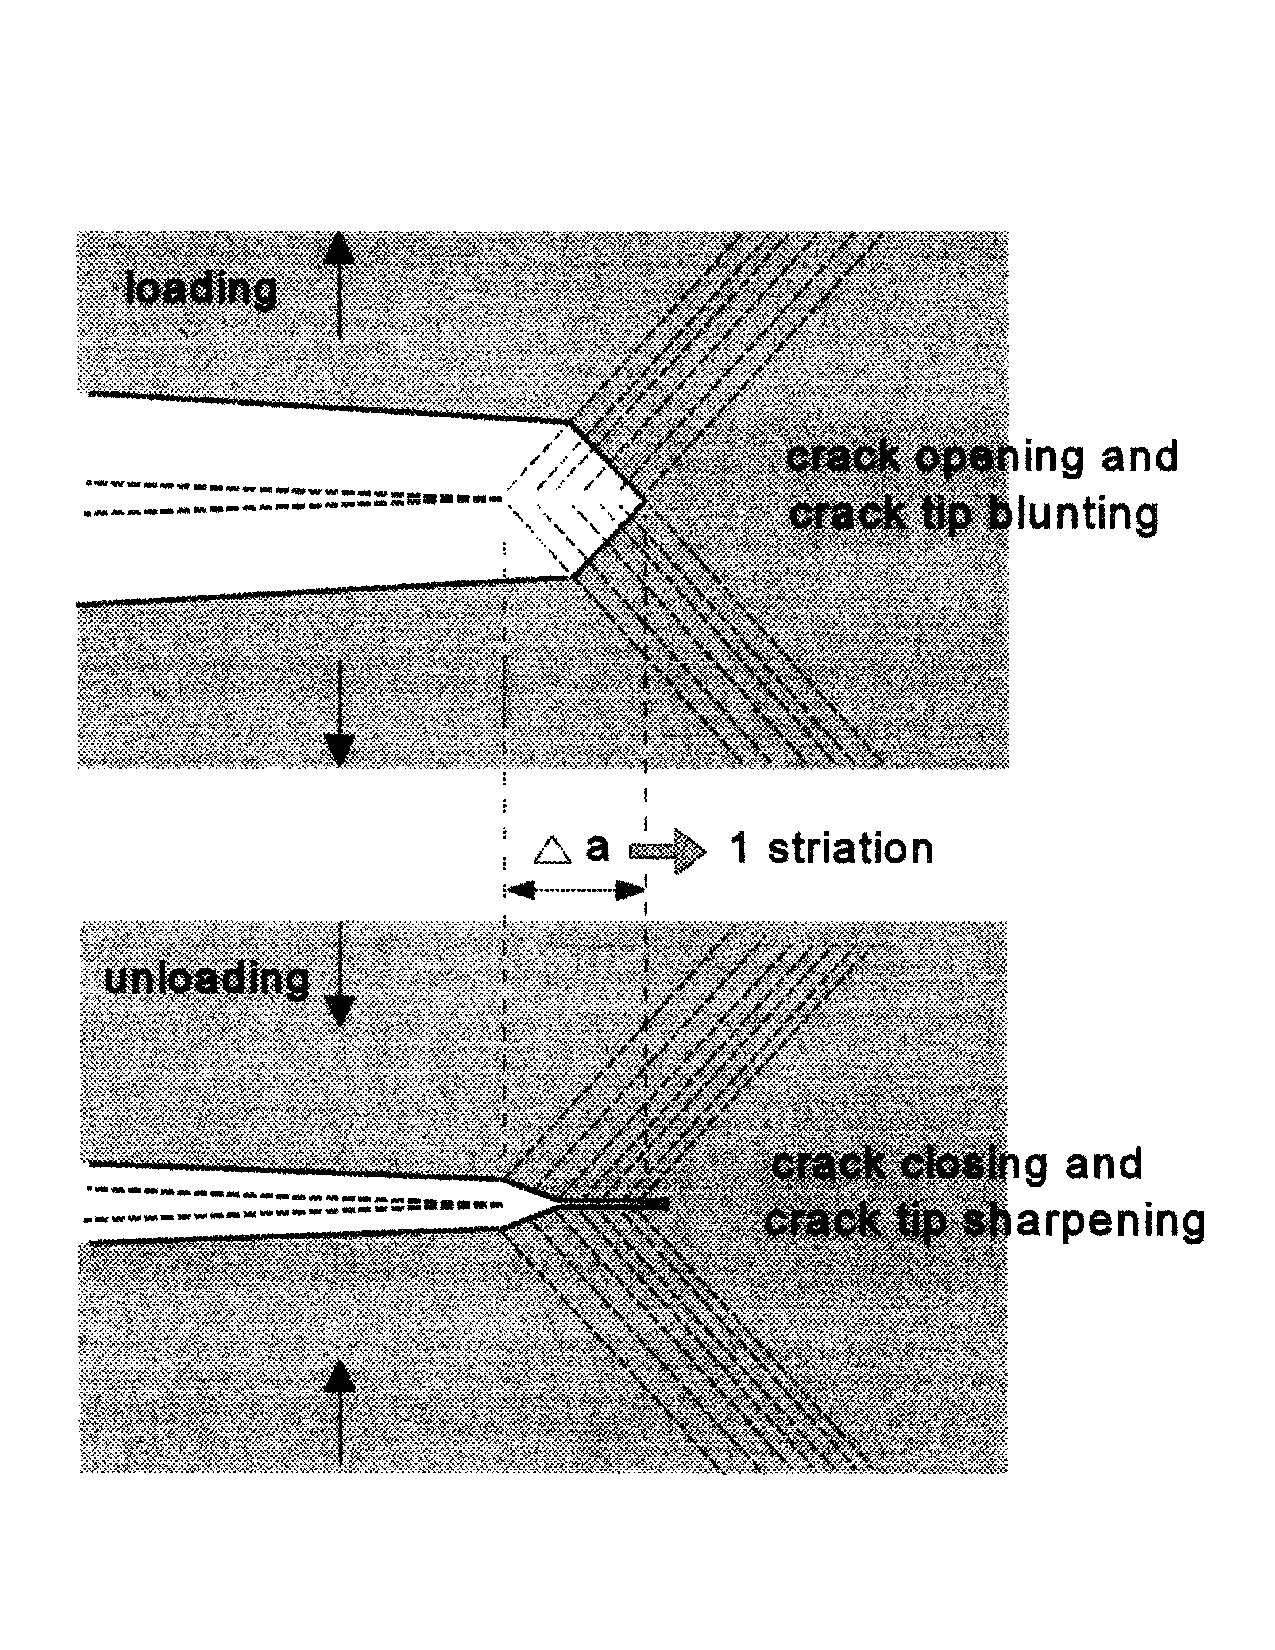
\includegraphics[width=0.5\linewidth, trim={0cm 2cm 0cm 3cm},clip]{Imagenes/crack_fatigue.pdf}
\caption{Crecimiento de una grieta durante un ciclo de carga perpendicular, dando origen a las marcas de playa. \cite{schijve2001fatigue}}
\label{fig:crack_fat}
\end{figure}

Finalmente, la última etapa es la falla del material, que ocurre en el último ciclo de la carga, al no poder soportarla con el material restante. Esta fractura es rápida y es producto de una macro-deformación plástica, pudiendo ser frágil, dúctil o una combinación de ambas.

Con esto en cuenta, es posible definir ciertos conceptos en base a las distintas etapas que experimenta un material. La vida a fatiga de un material (\textit{fatigue life}, $N_f$) es el número de ciclos aplicados a una probeta para lograr el criterio de falla \cite{ISO23718}. El límite de resistencia a la fatiga (\textit{endurance limit}) es frecuentemente explicado como la amplitud de esfuerzo para el cual la vida a fatiga tiende a infinito o a la asíntota de la curva S-N. Sin embargo, al comprender la fatiga como un proceso, es posible dar una definición más acertada para el límite a la fatiga, pasando a ser el umbral para el crecimiento de las microgrietas. Es decir, bajo este límite existe nucleación e iniciación de grites, sin embargo, su crecimiento está limitado a los bordes de grano del material.

Por otra parte, para el estudio de este fenómeno existen tres modelos de falla por fatiga: de \textit{esfuerzo-vida} ($S$-$N$), de \textit{deformación-vida }($\varepsilon$-N) y de la \textit{mecánica de fractura lineal elástica} (LEFM). Cada uno de ellos tiene ventajas y desventajas, sin embargo, la máquina que es objeto de evaluación en este trabajo utiliza el método \textit{esfuerzo-vida}. El criterio de elección entre los distintos modelos se divide principalmente por la cantidad de ciclos que se harán en la medición, los que se clasifican en régimen de fatiga de bajo ciclaje (\textit{low-cycle fatigue}, LCF) o un régimen de fatiga de alto ciclaje (\textit{high-cycle fatigue}, HCF). La división entre ambas se establece, por lo general, como $10^3 \leq$ \textit{LCF} y $10^3 >$ \textit{HCF} \cite{budynas2008shigley} (ver fig. \ref{fig:lcf_hcf}), debido a que la zona LCF está asociada a la existencia de macro-deformaciones plásticas en cada ciclo. De esta manera, el método de esfuerzo-vida se utiliza para ensayos de alto ciclaje debido a su poca precisión en casos LCF. A su vez, los métodos de deformación-vida y LEFM se aplican para casos LCF.

En el método de esfuerzo-vida las muestras o probetas son sometidas a fuerzas de magnitudes especificas, al mismo tiempo que se cuentan la cantidad de ciclos. Es por esto que es un modelo con base en el esfuerzo, con el cual se busca determinar un límite de resistencia a la fatiga. 

Estas fuerzas especificas pueden ser constantes o variables en el tiempo y magnitud, sin embargo, se abordará principalmente los casos donde los esfuerzos fluctúan de manera constante en el tiempo y de una amplitud fija debido a las características de la máquina analizada en este trabajo. Esto permite trazar la curva de fatiga $S$-$N$ del componente o material para distintas cargas con su respectivo número de ciclos en el que falla.

Por esto, se hace necesario describir y definir conceptos que surgen producto de una carga cíclica. Esta curva se caracteriza por el esfuerzo alternante (\textit{alternate stress} o \textit{amplitude stress}, $\sigma_a$) y el esfuerzo medio (\textit{mean stress}, $\sigma_m$) que se muestran en la ecuación \ref{eq:s_a} y \ref{eq:s_m}, respectivamente. A su vez, estas se definen por el esfuerzo máximo $\sigma_{max}$ y $\sigma_{min}$, siendo el esfuerzo máximo y mínimo alcanzado por la carga cíclica. Finalmente, el rango del esfuerzo, $\Delta \sigma$ o $\sigma_r$ (ec. \ref{eq:ds}), y la razón de esfuerzos, $R$ (ec. \ref{eq:r_s}), también son opciones  para caracterizar la fatiga.

\begin{align}
	\sigma_a &= \frac{\sigma_{max} - \sigma_{min}}{2} \label{eq:s_a} \\
	\sigma_m &= \frac{\sigma_{max} + \sigma_{min}}{2} \label{eq:s_m} \\
	\Delta \sigma &= \sigma_{max} - \sigma_{min} = 2\sigma_a  \label{eq:ds} \\
	R &= \frac{\sigma_{min}}{\sigma_{max}} \label{eq:r_s} 
\end{align}

Estos términos se pueden ver claramente en la fig. \ref{fig:defesf_fat}.

\newpage

Existen dos casos específicos destacables, el primero en donde $\sigma_m = 0$, y así $R=-1$, se llama esfuerzo de ciclo invertido. El segundo, cuando $\sigma_{min}=0$, y $R=0$, se llama esfuerzo repetido.

\begin{figure}[h]
\centering
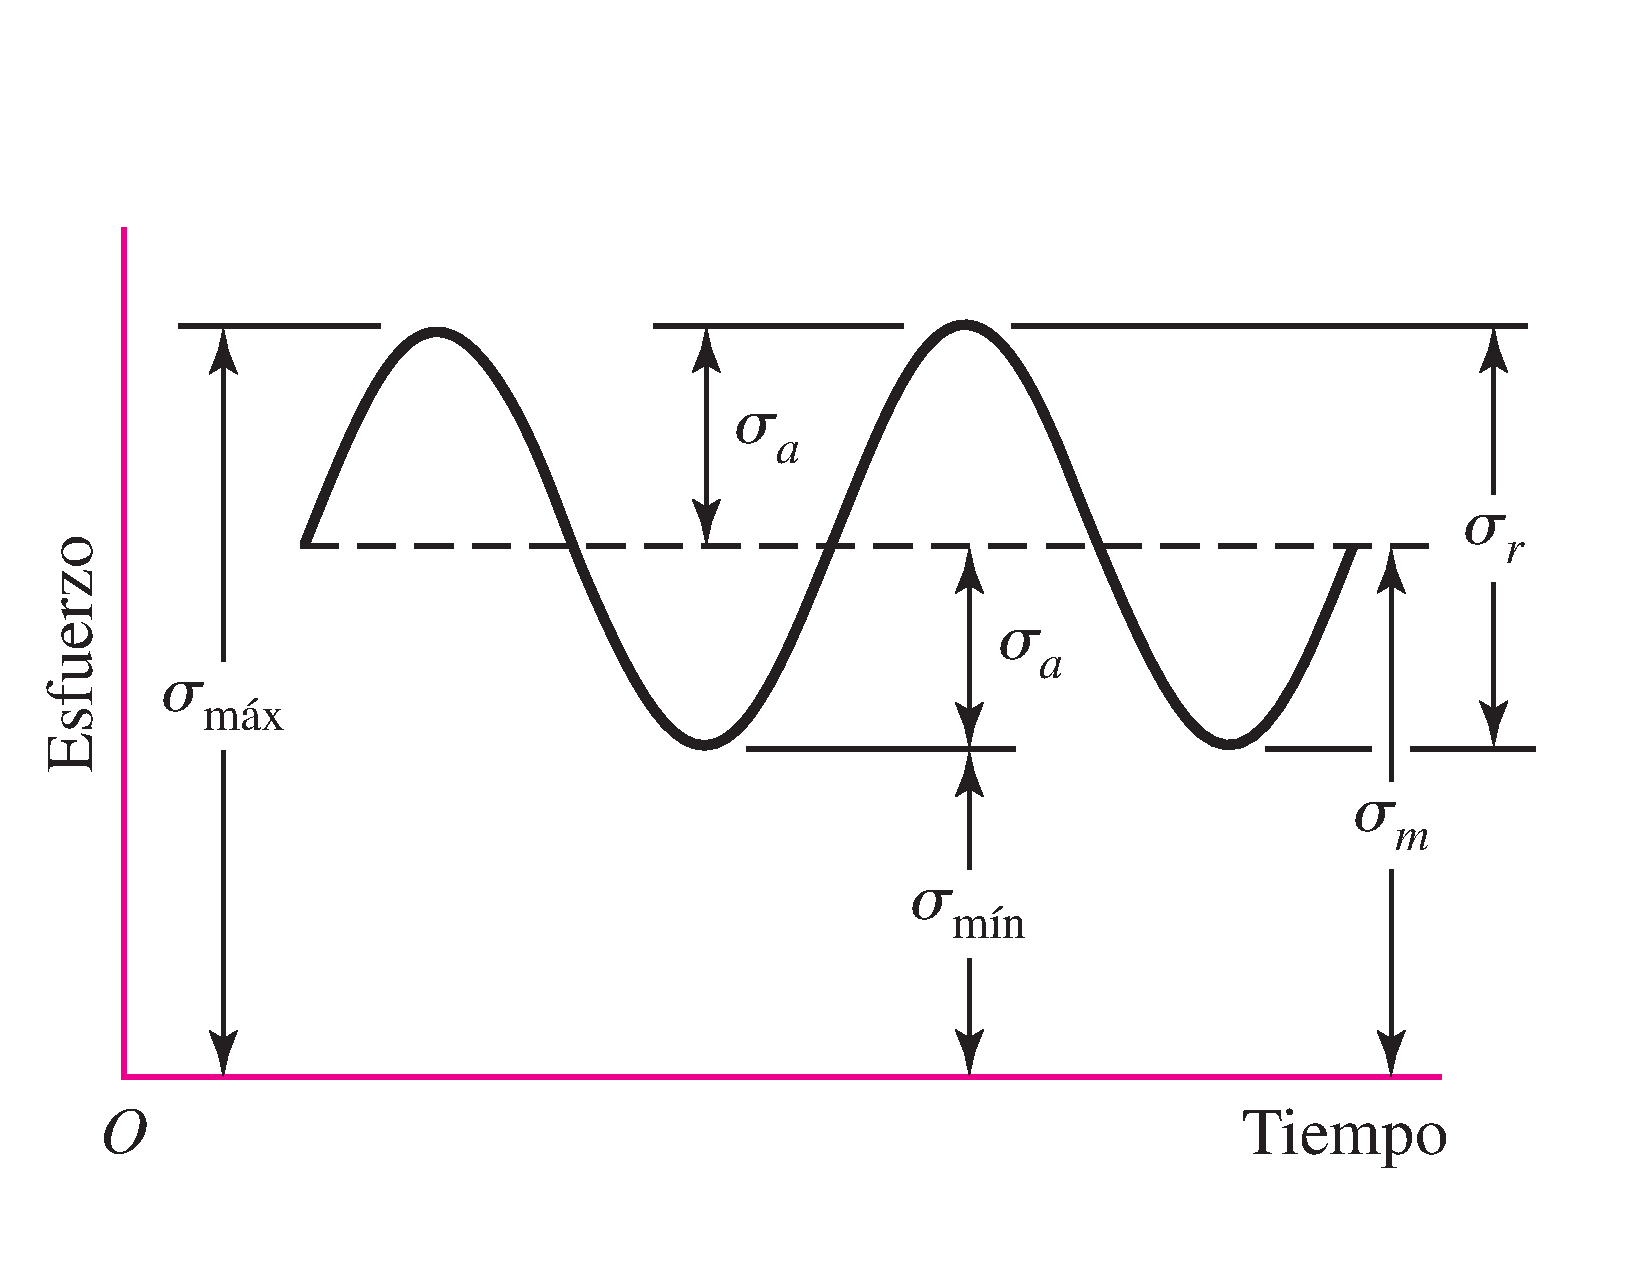
\includegraphics[width=0.6\linewidth, trim={0cm 1cm 0cm 2cm},clip]{Imagenes/defesf_fat.pdf}
\caption{Definición de los esfuerzos alternantes, máximo, mínimo y medio. \cite{budynas2008shigley}}
\label{fig:defesf_fat}
\end{figure}

\subsection{Curva S-N o de Wöhler}
Como se señaló en el punto anterior, la curva $S$-$N$ es el resultado de la aplicación del método esfuerzo-vida. Es quizás uno de las herramientas más importantes en el desarrollo empírico para lograr cuantificar el proceso de fatiga y poder diseñar contra este. El diagrama $S$-$N$ se obtiene como resultado de un número de ensayos de fatiga a distintos niveles de esfuerzo, donde $S$ puede ser la amplitud ($S_a$), el rango de esfuerzo ($\Delta S$) o el esfuerzo máximo ($S_{max}$) que es aplicado a la probeta, siendo la amplitud lo más común. La variable $N$ hace referencia a la vida a fatiga del material, es decir, la cantidad de ciclos hasta que la probeta falle. Debido a que se desea analizar fallas en LCF y HCF, la cantidad de ciclos necesarios para fallar la probeta pueden llegar a ser demasiado altos, por esto, $N$ se grafica en escala logarítmica.

La cantidad de ensayos requeridos para construir la curva $S$-$N$ dependerá de distintos factores como, por ejemplo, la confiabilidad esperada, el uso final de la información o de los recursos disponibles. La norma E739-10 -- "Statistical Analysis of Linear or Linearized Stress-Life ($S$-$N$) and Strain-Life ($\varepsilon$-$N$) Fatigue Data" \cite{E739} , establece una guía dependiendo del tipo de prueba a realizar como se muestra en al tabla \ref{tab:type_test}. Además, se recomienda realizar la medición con al menos tres puntos de esfuerzos distintos. Con esto, es posible obtener el diagrama $S$-$N$ como el que se aprecia en la fig. \ref{fig:lcf_hcf}, donde se puede notar la diferencia entre la zona LCF, HCF y de vida infinita.

\begin{table}[h]
\begin{center}
\begin{tabular}{@{}lc@{}}
\toprule
\multicolumn{1}{c}{Tipo de prueba}                                                                                        & Cantidad mínima de probetas \\ \midrule
\begin{tabular}[c]{@{}l@{}}Preliminar y exploratorio (investigación exploratoria \\ y ensayos de desarrollo)\end{tabular} & 6 a 12                      \\
\begin{tabular}[c]{@{}l@{}}Pruebas de desarrollo e investigación de componentes \\ y probetas\end{tabular}                & 6 a 12                      \\
Datos de diseños permisibles                                                                                              & 12 a 24                     \\
Datos de confiabilidad                                                                                                    & 12 a 24                     \\ \bottomrule   
\end{tabular}
\caption{Número mínimo de pruebas según tipo de prueba. \cite{E739}}
\label{tab:type_test}
\end{center}
\end{table}

\begin{figure}[h]
\centering
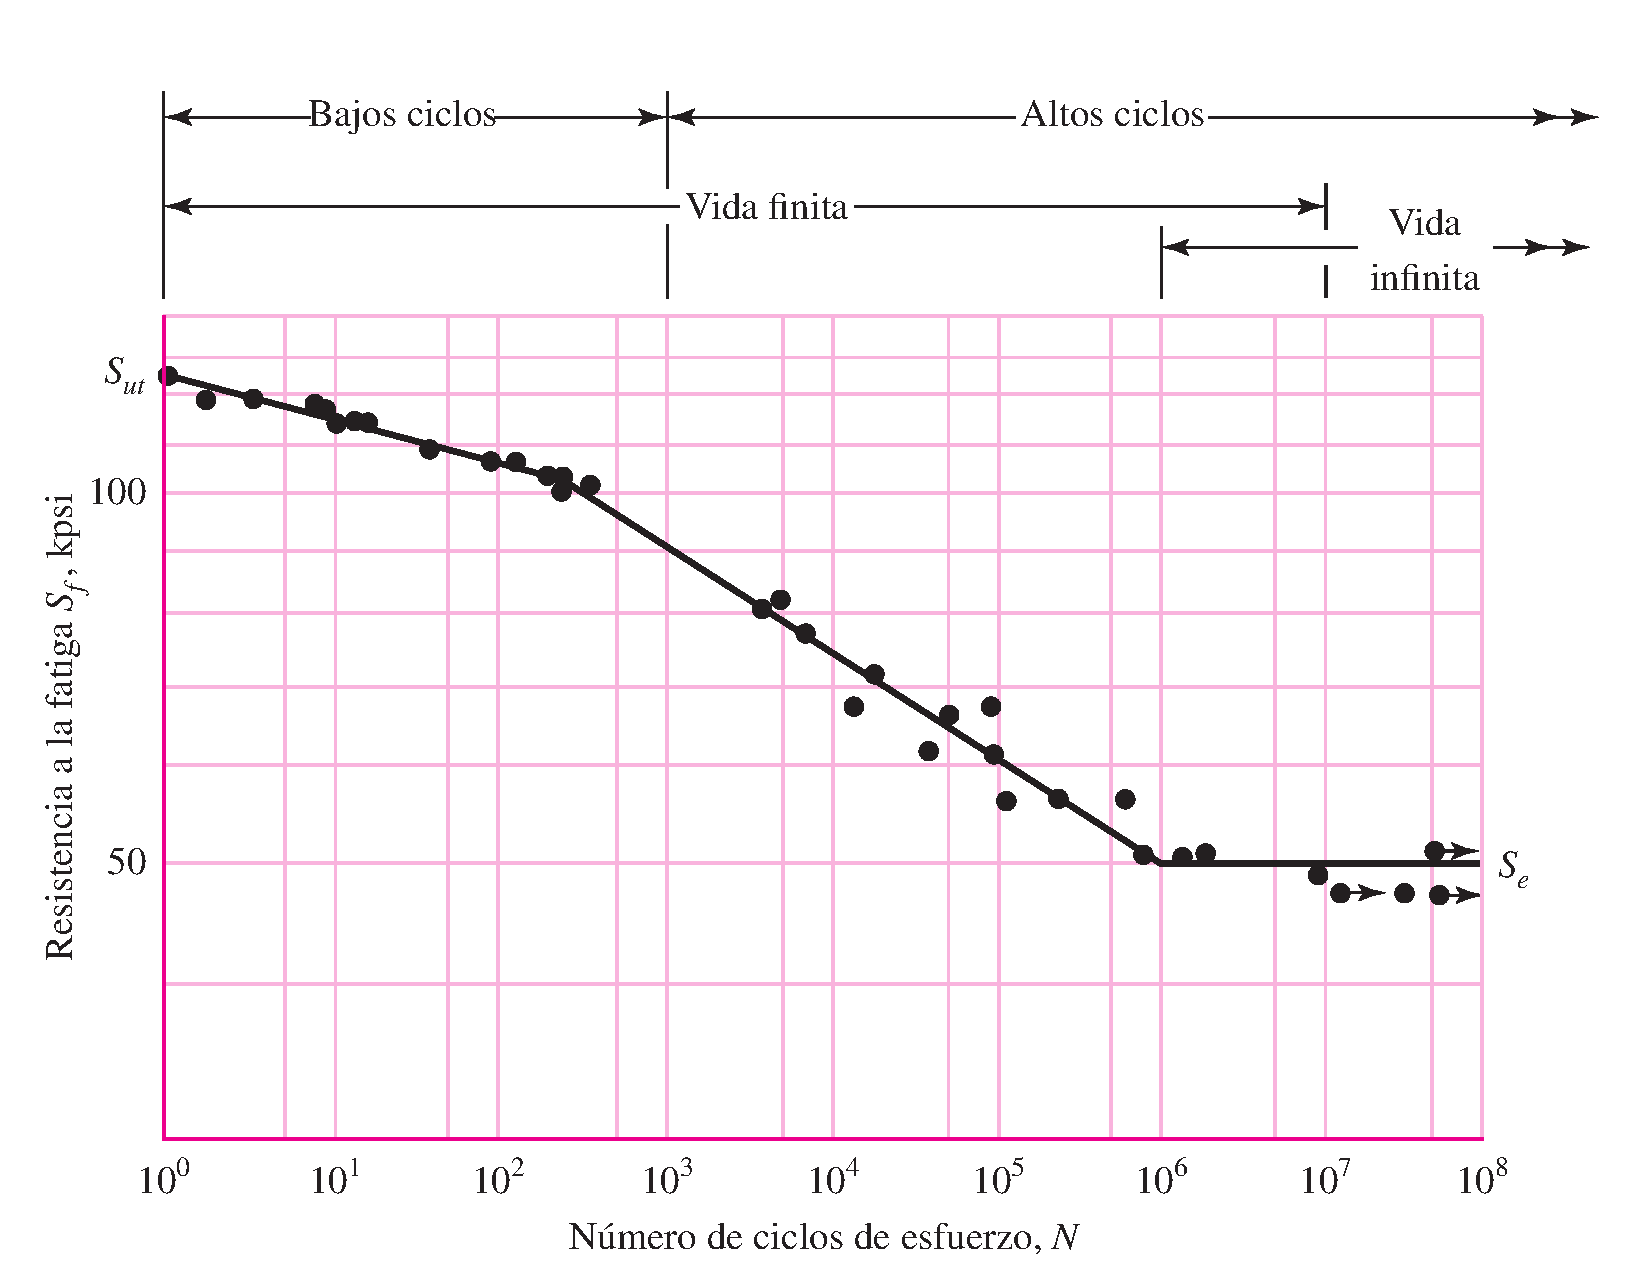
\includegraphics[width=0.75\linewidth]{Imagenes/lcf_hcf.pdf}
\caption{Diagrama $S$-$N$ obtenido a partir de los resultados de ensayos a fatiga axial con carga invertida. Se pueden apreciar las zonas LCF, HCF y la zona de vida infinita. \cite{budynas2008shigley}}
\label{fig:lcf_hcf}
\end{figure}

La curva $S$-$N$ varía ámpliamente sus resultados para distintos tipos de materiales y, a su vez, estos se ven afectados por una variedad de factores. Estos pueden ser por modificaciones en las condiciones de ensayo, de la geometría de la probeta, de la naturaleza del material o de la forma de fabricación de la probeta. Todos estos factores crean ciertas tendencias en la obtención de datos que los distinguen unos de otros. 

En concreto, las condiciones medioambientales hostiles, ya sean químicas o térmicas, pueden acelerar el proceso de iniciación y crecimiento de grietas. Una probeta sometida a creep, fatiga y altas temperaturas puede disminuir drásticamente sus vida útil y, por tanto, la vida a fatiga del material. También es posible realizar ensayos en una solución de sal para homologar las condiciones marinas, afectando su vida a fatiga. Otro factor que afecta los resultados de los ensayos es la frecuencia de los ciclos de carga ejercidos, al aumentar la temperatura de la probeta durante su ensayo.

El esfuerzo residual también tiene incidencia en la curva de Wöhler, la cual puede incluso ser beneficiosa al utilizar técnicas como el granallado (\textit{shot peening}). El mecánizado de las piezas, como en el caso de la probeta utilizada por la máquina de fatiga, verá afectado los resultados de la curva $S$-$N$ dependiendo de las características con las que sea manufacturado. Como se indicó anteriormente, la primera etapa de la fatiga, la iniciación de las grietas, es un fenómeno que depende de la superficie del material y como consecuencia, un mecanizado grueso o fino tendrá un impacto en esa etapa de la fatiga y no en la posterior. Así, aquellas probetas que tengan una mejor calidad superficial producto del afinado, tendrán una mejor resistencia a la fatiga respecto a otras.

Es posible encontrar otros factores que inciden en los resultados de la curva, como pueden ser la geometría de la probeta o componente, sus dimensiones, el esfuerzo último ($\sigma_{u}$), su microestructura, tratamientos químicos y el esfuerzo medio ($S_m$). Este último será analizado en la sección siguiente, debido a la importancia que posee al estar presente en la máquina que se estudia en este trabajo.

\subsection{Esfuerzo medio, $S_m$}
Como se escribió anteriormente, el esfuerzo medio tiene influencia en el resultado de una curva $S$-$N$, disminuyendo el límite a la resistencia de la fatiga del material a medida que aumenta su carga media. Debido a que realizar ensayos para cada carga media resultaría muy costoso, existen ecuaciones que buscan estimar el efecto de un esfuerzo sobre un material o componente. 

\begin{figure}[h]
\centering
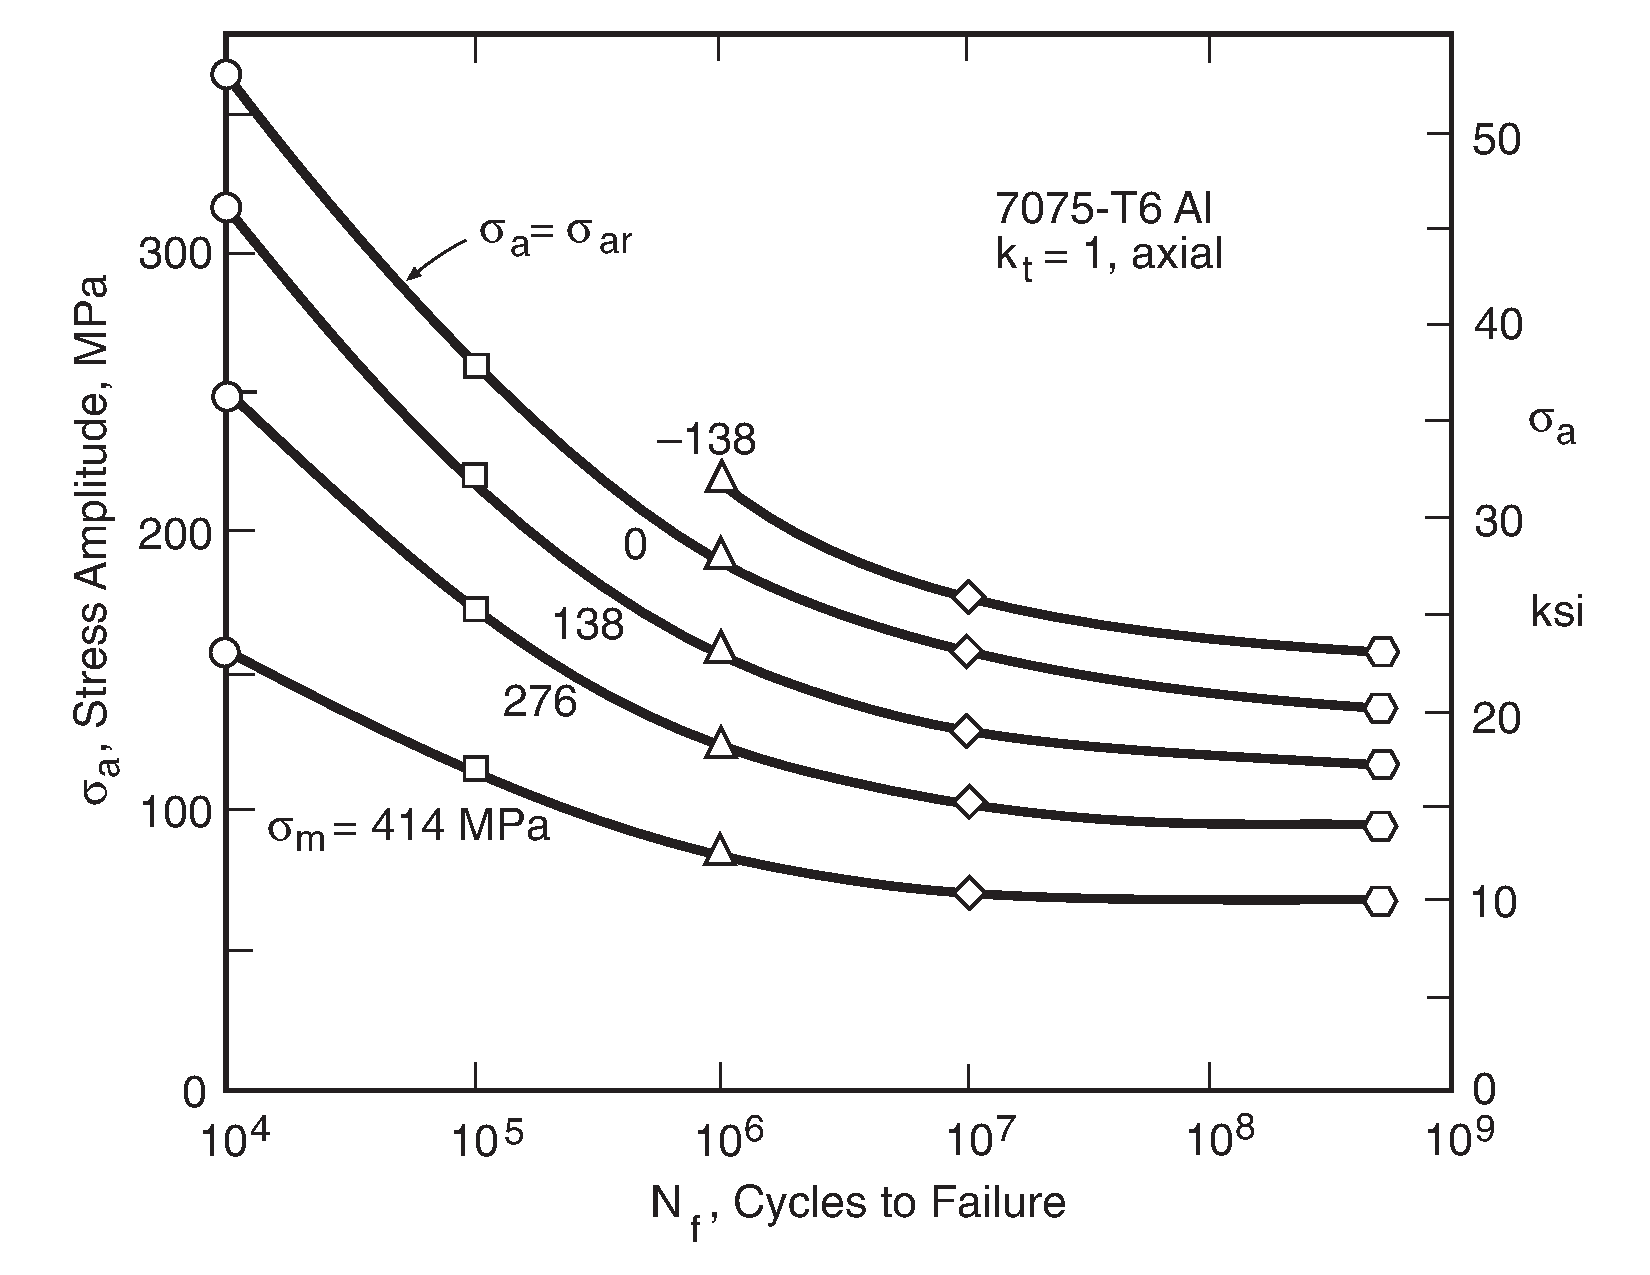
\includegraphics[width=0.6\textwidth]{Imagenes/s_n_mean.pdf}
\caption{Diagrama $S$-$N$ de ensayos de fatiga axial con distintos esfuerzos medios para aluminio 7075-T6. \cite{dowling2013mechanical}}
\label{fig:s_n_mean}
\end{figure}

Se utilizan distintas maneras para representar la información de un ensayo cuando $S_m \neq 0$. Una forma es recolectar la información de distintos ensayos con distintos valores de carga media y graficarlos como se muestra en la fig. \ref{fig:s_n_mean}. Una segunda opción es realizar un diagrama de vida constante (\textit{constant fatigue life diagram}, \textit{CFL}), mostrada en la fig. \ref{fig:diag_cfl}, el cual muestra claramente que un incremento del esfuerzo medio tiene como resultado una disminución del esfuerzo alternante, para la misma vida de la probeta, $N_f$.

\begin{figure}[h]
\centering
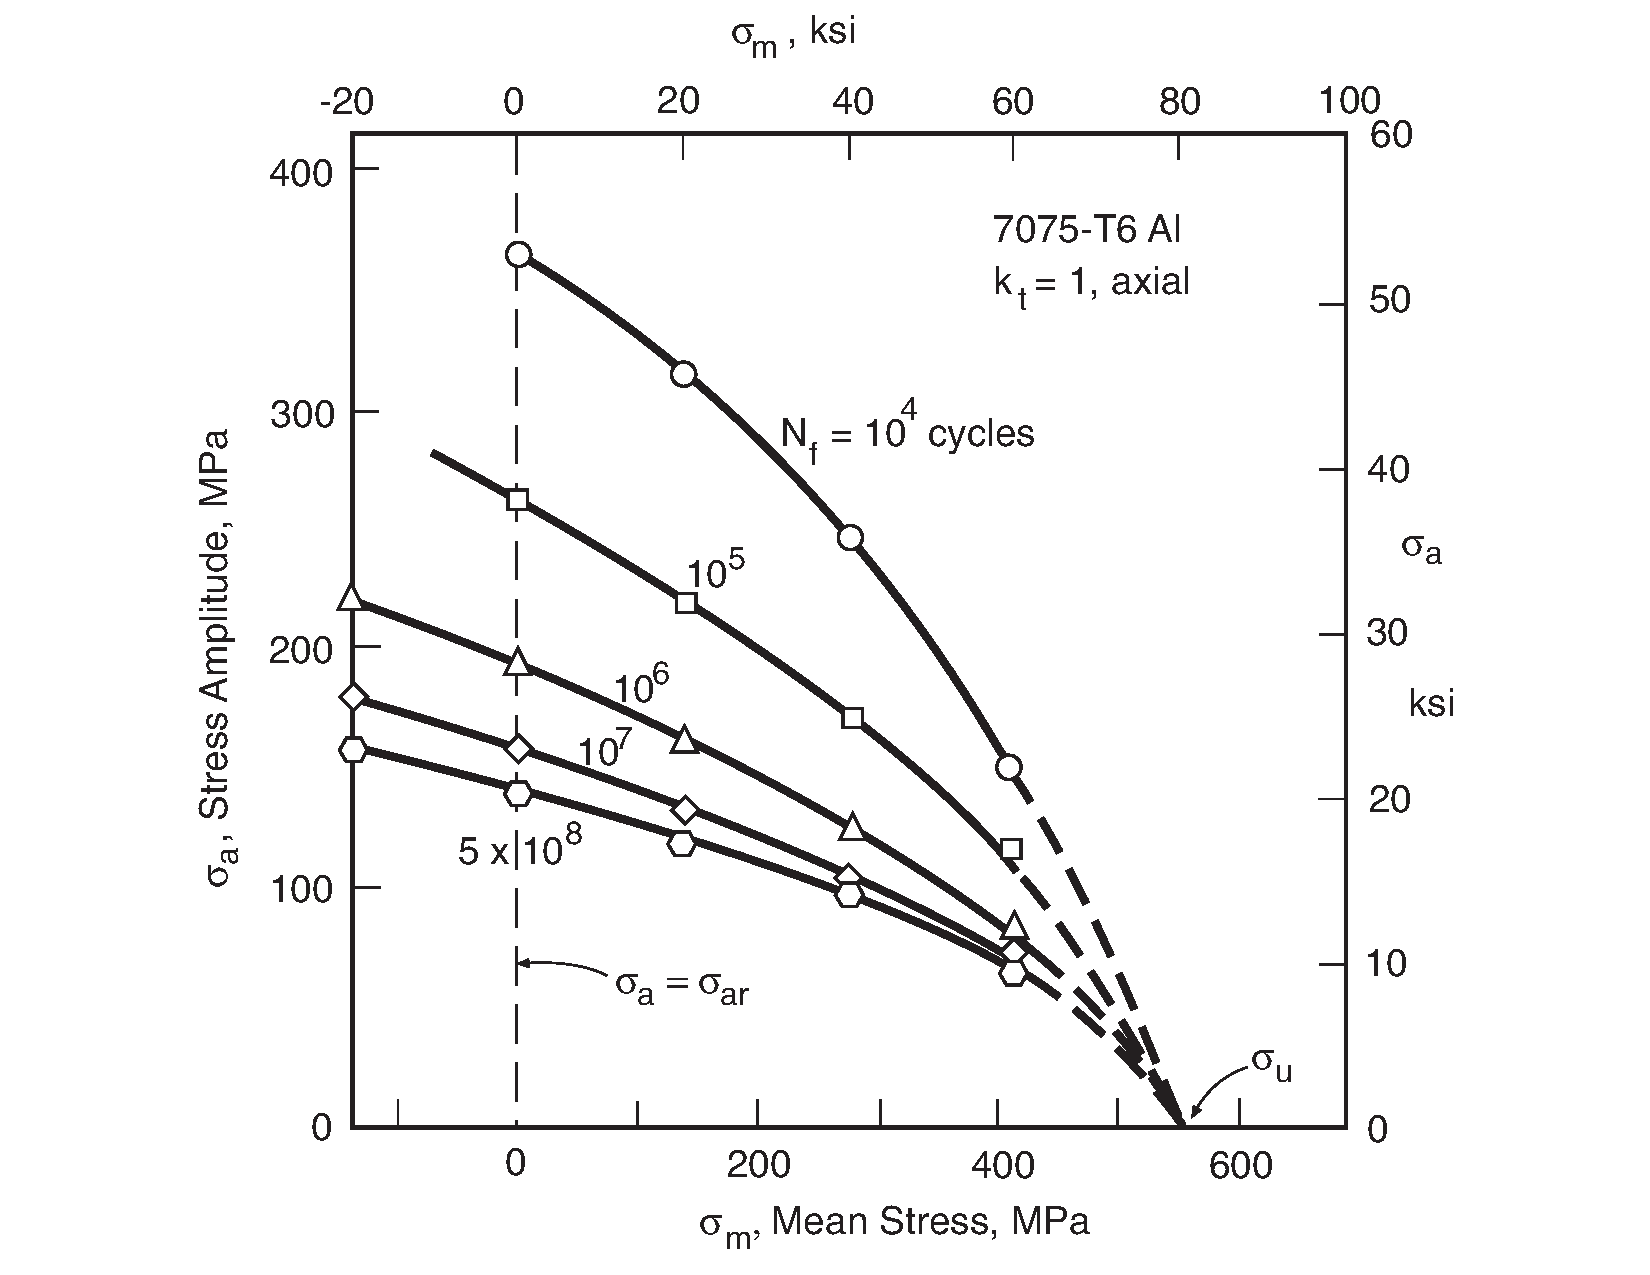
\includegraphics[width=0.7\textwidth]{Imagenes/diag_cfl.pdf}
\caption{Diagrama de vida constante para aluminio 7075-T6. \cite{dowling2013mechanical}}
\label{fig:diag_cfl}
\end{figure}

\newpage

\subsection{Diseño para esfuerzos uniaxiales fluctuantes}
Es importante tomar en consideración en el diseño de elementos la componente media de la carga fluctuante. Para esto, se utiliza un diagrama de esfuerzo alternante versus esfuerzo normal en el cual se ajustan distintas curvas a los datos obtenidos. Como se muestra en la fig. \ref{fig:falla_fat}, existe la línea de Goodman modificada, la parábola de Gerber y la línea de Soderberg. 

\begin{figure}[h]
\centering
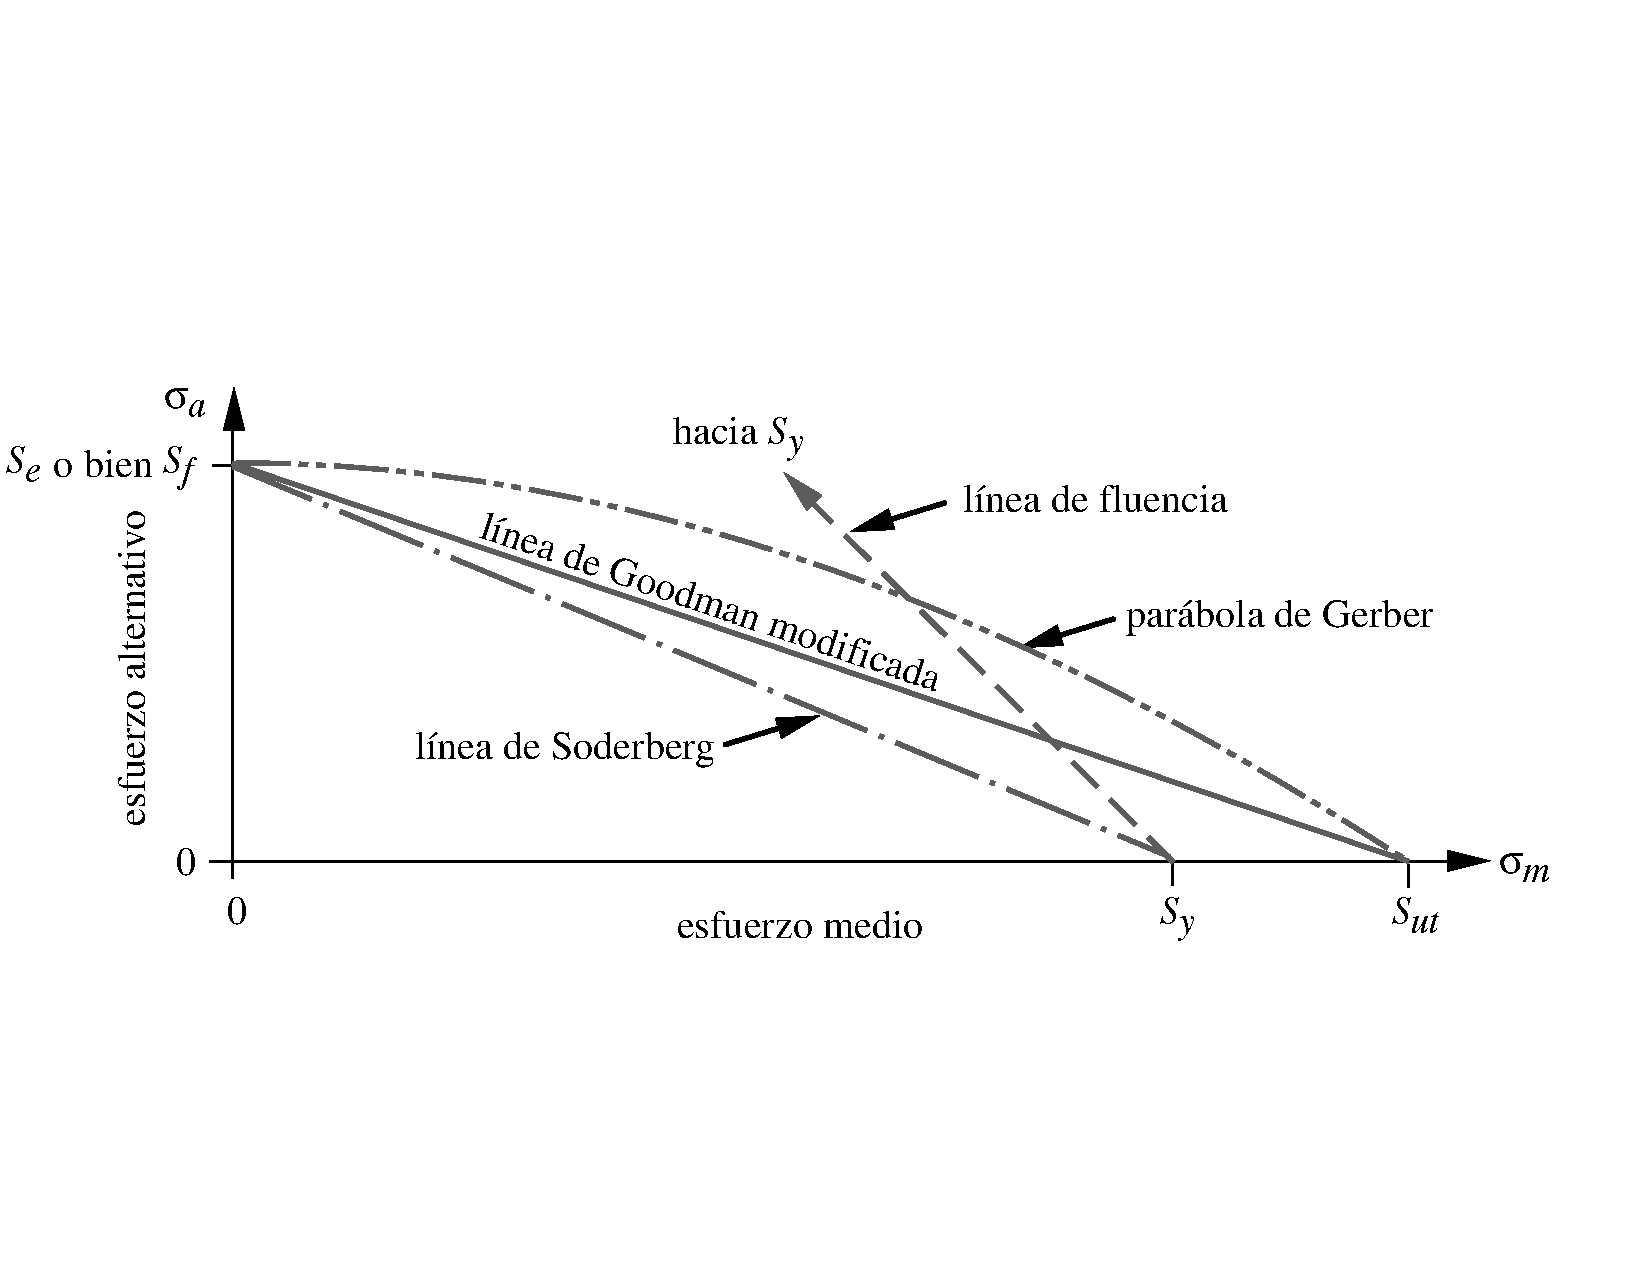
\includegraphics[width=0.8\linewidth, trim={0cm 4.5cm 0cm 5.5cm},clip]{Imagenes/falla_fat.pdf}
\caption{Curvas de estimación de falla a fatiga de Goodman, Gerber y Soderberg.\cite{norton2011machine}}
\label{fig:falla_fat}
\end{figure}

La parábola de Gerber es la que mejor se ajusta a los datos de falla experimental, de acuerdo a la ec. \ref{eq:gerber}; mientras que la línea de Goodman modificada, ec. \ref{eq:good_mod}, se ajusta por debajo de la dispersión de datos. Ambas curvas utilizan en el eje $\sigma_a$ el límite de resistencia a la fatiga $S_e$ y el esfuerzo último $S_u$ en el eje $\sigma_m$. En cambio, la línea de Soderberg, ec. \ref{eq:soderberg}, une $S_e$ con la resistencia a la fluencia del material $S_y$ y es, por lo tanto, un criterio de falla más conservador que los demás. Sin embargo, la línea punteada que une ambos $S_y$ se debe utilizar en las dos primeras curvas como límite del primer ciclo de esfuerzo para evitar que ceda o falle. \cite{norton2011machine}

\begin{centering}
\begin{align}
&\text{Parábola de Gerber:}&	\frac{\sigma_a}{S_e} &+ \frac{\sigma_m^2}{S_u^2} = 1 \label{eq:gerber}\\
&\text{Goodman modificada:}&	\frac{\sigma_a}{S_e} &+ \frac{\sigma_m}{S_u} = 1 \label{eq:good_mod}\\
&\text{Soderberg:}&	\frac{\sigma_a}{S_e} &+ \frac{\sigma_m}{S_y} = 1 \label{eq:soderberg}
\end{align}
\end{centering}

\subsubsection{Diagramas de esfuerzos alternantes normalizados y medios}

La normalización del diagrama mostrado en la fig. \ref{fig:diag_cfl} responde a la necesidad de consolidar los datos de mediciones para distintos esfuerzos medios y vida de fatiga dentro una sola curva. Esto da la oportunidad de ajustar la curva a una ecuación que represente todos los datos obtenidos. Así para el caso particular de $S_m=0$, el esfuerzo alternante se designará por $\sigma_{ar}$. Por lo tanto, en el diagrama \textit{CFL}, $\sigma_{ar}$ es el intercepto en $\sigma_m=0$ de la curva para cualquier vida $N_f$. Por consiguiente, el gráfico puede ser normalizado utilizando la relación $\sigma_a/\sigma_{ar}$ en la ordenada y el esfuerzo medio $\sigma_m$ en la abscisa. De esta manera, se cumplirá que $\sigma_a/\sigma_{ar}=1$ cuando $\sigma_m=0$ y, además, cuando el esfuerzo alternante es cercano a cero, el valor del esfuerzo medio debe aproximarse al esfuerzo último del material, $\sigma_u$. El resultado de esto se puede apreciar en la fig. \ref{fig:cfl_norm}.

\begin{figure}[h]
\centering
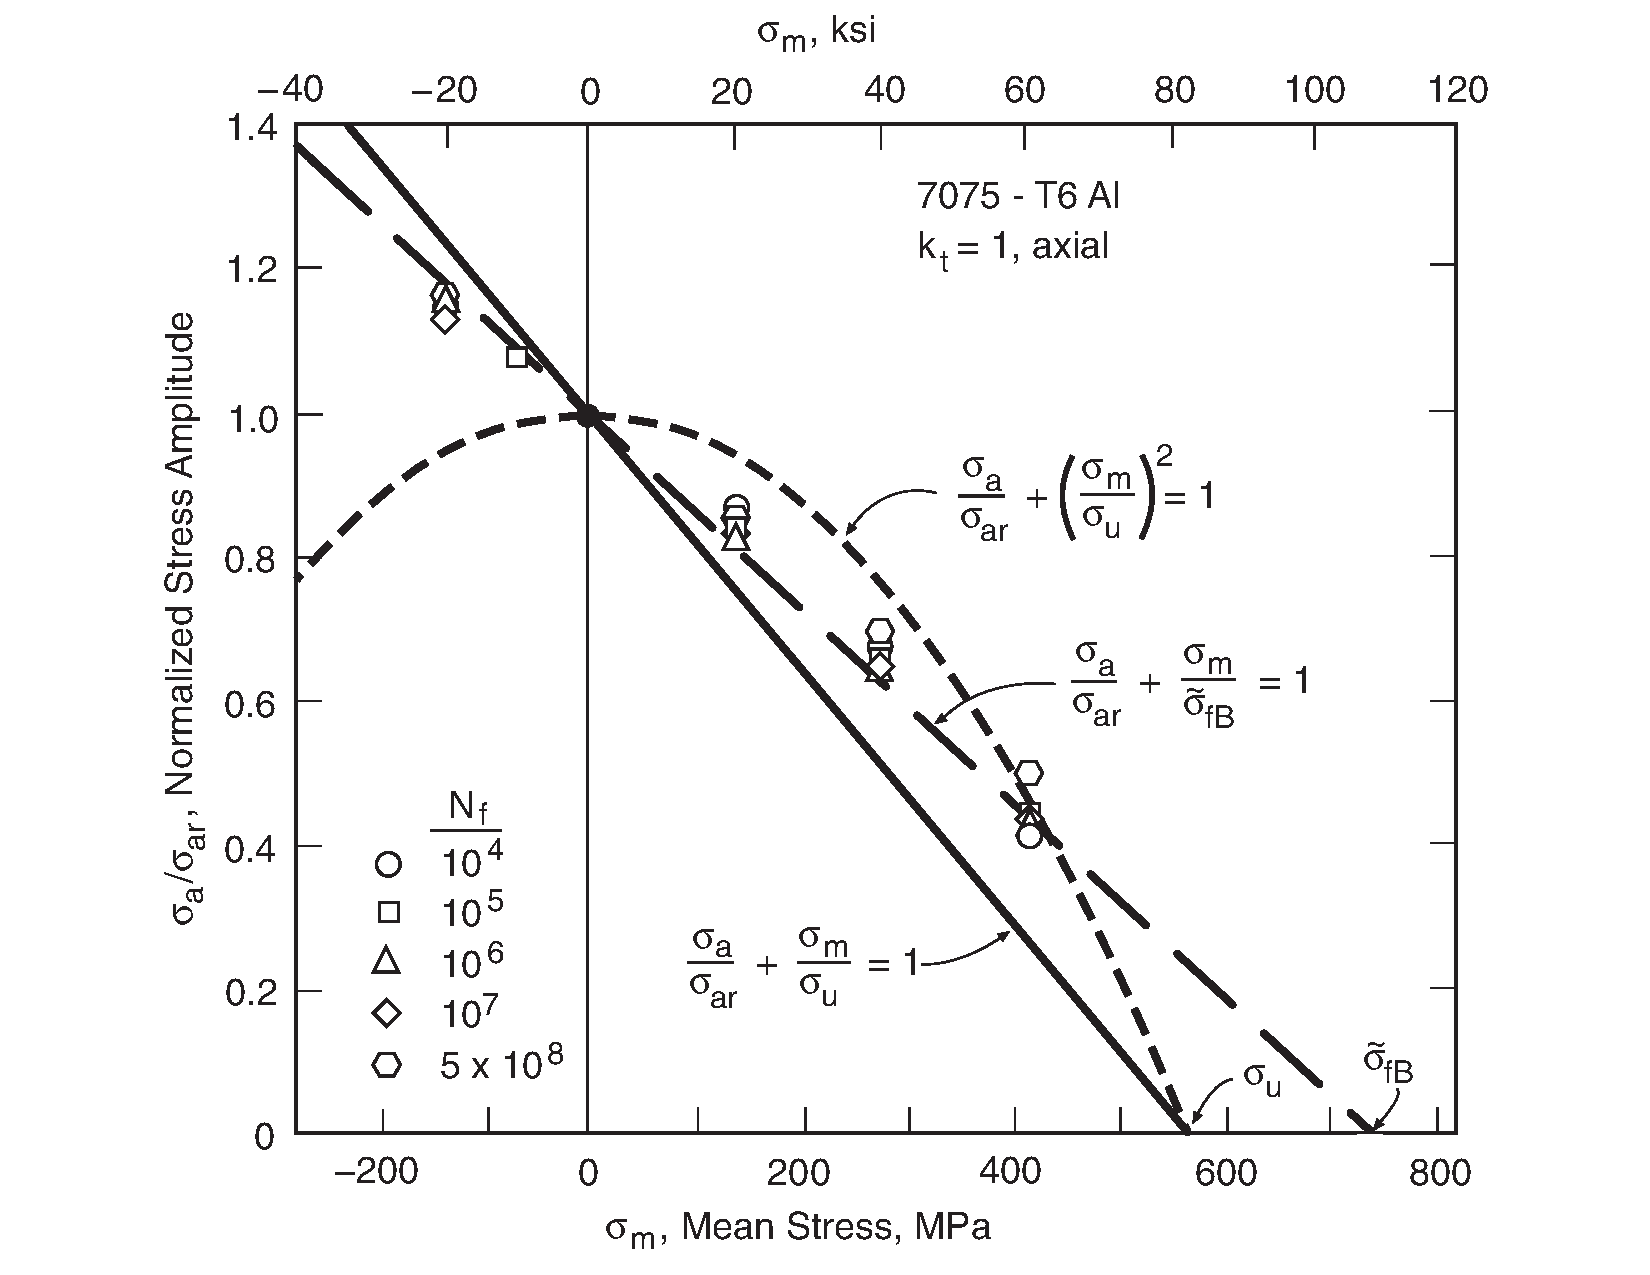
\includegraphics[width=0.7\textwidth]{Imagenes/cfl_norm.pdf}
\caption{Diagrama \textit{CFL} normalizado para aluminio 7075-T6. \cite{dowling2013mechanical}}
\label{fig:cfl_norm}
\end{figure}

Al igual a como se vio en la sección anterior, las curvas que se ajustan a estos valores pueden ser rectas o una parábola. La ecuación modificada de Goodman normalizada sigue siendo una aproximación conservadora, y su versión normalizada es:

\begin{equation} \label{eq:good_norm}
	\frac{\sigma_a}{\sigma_{ar}} + \frac{\sigma_m}{\sigma_u} = 1 
\end{equation}

La parábola de Gerber queda expresada como:

\begin{equation} \label{eq:par_gerber}
	\frac{\sigma_a}{\sigma_{ar}} + \left(\frac{\sigma_m}{\sigma_u}\right)^2 = 1 
\end{equation}

Y una segunda modificación de la ecuación de Goodman, propuesta por J. Morrow, para metales dúctiles, en la cual se reemplaza $\sigma_u$ por el esfuerzo verdadero de fractura corregido $\tilde{\sigma}_{fB}$.

\begin{equation} \label{eq:mod_goodduct}
	\frac{\sigma_a}{\sigma_{ar}} + \frac{\sigma_m}{\tilde{\sigma}_{fB}} = 1 
\end{equation}

\newpage

\section{Dinámica}

El movimiento y la relación existente entre las fuerzas que actúan sobre un cuerpo rígido es estudiado por la dinámica, la cual busca predecir el movimiento y explicar su origen. 

\subsection{Ecuaciones de movimiento de un cuerpo rígido}
\label{sec:ec_mov}
Para describir el movimiento de un cuerpo es necesario recurrir a la segunda ley de movimiento de Newton, la cual permite trazar y predecir el movimiento de traslación y rotación del cuerpo.

Si sobre una masa $m$ constante actúa una fuerza $\vec{F}(t)$ que da como resultado un vector de desplazamiento $\vec{x}(t)$, la segunda ley de Newton se expresa:
\begin{equation}\label{eq:newton_lineal}
	\vec{F}(t) = \frac{d}{dt}\left(m\frac{d\vec{x}(t)}{dt}\right) = m \frac{d^2\vec{x}(t)}{dt^2}
\end{equation}
De manera análoga para el mismo cuerpo rígido, de momento de inercia $I$, es sometido a un momento $\vec{M}(t)$, entonces el cuerpo girará con un vector de desplazamiento angular $\vec{\theta}$.
\begin{equation}\label{eq:newton_angular}
	\vec{M}(t) = I\frac{d^2\vec{\theta}(t)}{dt^2}
\end{equation} 
Con las ecuaciones \ref{eq:newton_lineal} y \ref{eq:newton_angular} se puede describir el movimiento plano de un sólido rígido.

Por otro lado, el principio de D\texttt{'}\kern-0.3em Alembert nos permite establecer un equilibrio dinámico entre las suma de las fuerzas externas o momentos y el producto entre su masa y la aceleración resultante del sólido, que se le denominará fuerza efectiva. Ambos términos deben ser equipolentes sobre el sistema que actúan, de esta manera las ecuaciones \ref{eq:2l_newton} y \ref{eq:2l_euler} son el resultado de la aplicación de este principio.
\begin{gather}
	\sum \mathbf{F_i} = m\mathbf{\ddot{x_i}} \label{eq:2l_newton}\\
	\nonumber \\
	\sum \mathbf{M_i} = I\mathbf{\ddot{\theta_i}} \label{eq:2l_euler}
\end{gather}

\subsection{Energía cinética de un cuerpo rígido}
Un cuerpo rígido en movimiento tiene asociada una energía cinética que depende de su masa $m$, el momento de inercia $I$, su velocidad $v$ y la velocidad de rotación $\omega$. Así la energía cinética $T$ queda definida por la ec. \ref{eq:e_cinetica}.
\begin{equation}\label{eq:e_cinetica}
	T = \frac{1}{2}mv^2 + \frac{1}{2}I\omega^2 
\end{equation}


\section{Vibraciones}
Es el estudio del movimiento repetitivo de los objetos relativo a un marco de referencia estacionario y que oscila respecto a una posición nominal. Es un fenómeno que se da en todos los objetos, afectando naturalmente el diseño en ingeniería, pudiendo ser perjudicial o útil, dependiendo del objetivo que se busca. Por esto, es necesario conocer cabalmente el fenómeno de la vibración, es decir, saber como analizarlo, medirlo y controlarlo para poder manejar las distintas variables que lo afectan.

Físicamente, la vibración es la interacción entre la energía potencial y cinética. De esta manera, un sistema vibratorio debe tener un componente que almacene la energía y la libere en forma de movimiento de una masa para, asimismo, este vuelva a ser almacenado en forma de energía potencial. Los elementos que componen un sistema mecánico y los métodos para describir los movimientos se explicarán en esta sección.


\subsection{Rigidez}
El comportamiento como resorte se puede aplicar a distintos elementos y componentes, dependiendo de su geometría y las propiedades del material. Así, a partir de la configuración del sistema, es posible calcular una rigidez $k$ para el movimiento longitudinal, transversal o torsional. 

El cálculo de la constante de rigidez para una viga de área $A$, módulo de Young $E$, largo $L$ y el segundo momento de área $\bar{I}$, se puede obtener a través de las ecuaciones de energía. Así, la ec. \ref{eq:k_cantilever}, muestra el valor de $k$ para una viga en voladizo con una carga $P$ en su extremo.
\begin{equation}\label{eq:k_cantilever}
	k = \frac{3E\bar{I}}{L^3}
\end{equation}

Por otro lado, la ec. \ref{eq:e_potelas}, muestra la energía potencial elástica asociada a un elemento que se comporta como un resorte.
\begin{equation}\label{eq:e_potelas}
	U_k = \frac{1}{2}k\,x(t)
\end{equation}


\subsection{Damping}
\label{sec:damping}
Los sistemas vibratorios predicen oscilaciones indefinidas si solo se considera la rigidez del resorte y la masa del sistema, sin embargo, la experiencia nos indica que los sistemas tienden a eventualmente reducir su movimiento hasta cero si estos no están afectados por fuerzas externas. Para esto es necesario añadir un modelo físico para disipar la energía y amortiguar el sistema mecánico. Así, el modelo expresado anteriormente debe ser modificado para considerar la reducción de movimiento en el tiempo. Para esto, se añade a las ecuaciones diferenciales un término de la forma $c\dot{x}(t)$, donde $c$ es una constante, el cual da como resultado una solución donde $x(t)$ tiende a un punto de reposo. Este tipo de \textit{damping} se llama amortiguamiento viscoso, en el cual su fuerza ($f_c$) es proporcional a la velocidad del sistema en la dirección opuesta del movimiento. Por lo tanto, la ec. \ref{eq:f_damp} muestra la fuerza de amortiguamiento, de tipo viscoso, presente en un sistema mecánico.
\begin{equation}\label{eq:f_damp}
	f_c = c\dot{x}(t)
\end{equation}

Producto del amortiguamiento de la oscilación del sistema, la frecuencia es menor que la de un sistema no amortiguado, disminuyendo exponencialmente. A partir del valor de la constante $c$, existen tres casos posibles:
\begin{enumerate}
	\item \textbf{Subamortiguado}: El sistema continúa teniendo un movimiento oscilatorio, con un decaimiento exponencial de la amplitud hasta llegar a la posición de reposo.
	\item \textbf{Sobreamortiguado}: El movimiento del sistema no alcanza a ser oscilatorio, sin embargo, vuelve a la posición de reposo exponencialmente.
	\item \textbf{Críticamente amortiguado}: Es el caso que separa si el decaimiento es oscilatorio, siendo el movimiento que retorna al reposo más rápido sin oscilaciones.
\end{enumerate}

Por lo tanto, la ecuación que describe el movimiento de un sistema amortiguado es:
\begin{gather*}
	m\ddot{x} = -f_c - f_k \\
	m\ddot{x}(t) + c\dot{x}(t) + kx(t) = 0 
\end{gather*}

Desde la perspectiva del método de energía, el amortiguamiento viscoso es una fuerza no conservativa que puede ser modelada por la función de disipación de Rayleigh, que toma la forma \ref{eq:rayleigh_function}.
\begin{equation}\label{eq:rayleigh_function}
	R = \frac{1}{2}c\,\dot{q_i}^2
\end{equation} 
Si $q$ es cada coordenada generalizada y $n$ es el número de coordenadas generalizadas, entonces se pueden obtener las fuerzas generalizadas para amortiguamiento viscoso derivando $R$ respecto a cada variable generalizada $q$, como se muestra en la ec. \ref{eq:q_ri}.
\begin{equation}\label{eq:q_ri}
	Q_{Rj} = -\frac{\partial R}{\partial \dot{q_j}}, \; \text{para cada }\, j=1,2,...,n
\end{equation}

\subsection{Vibraciones forzadas}
\label{sec:vib_forzadas}
Los sistemas mecánicos están sometidos a una gama bastante amplia de fuerzas externas que actúan sobre ellos, las que pueden ser aleatorias, periódicas, no periódicas o transientes. La fuente puede ser variada, pero todas ellas causan vibraciones en el sistema, las cuales se denominarán $F(t)$. Para el caso de este trabajo, el sistema a analizar contiene un disco sometido a una velocidad de rotación constante, impulsado por un motor eléctrico, que produce una fuerza periódica producto de su desbalanceo.

\begin{figure}[h]
\centering
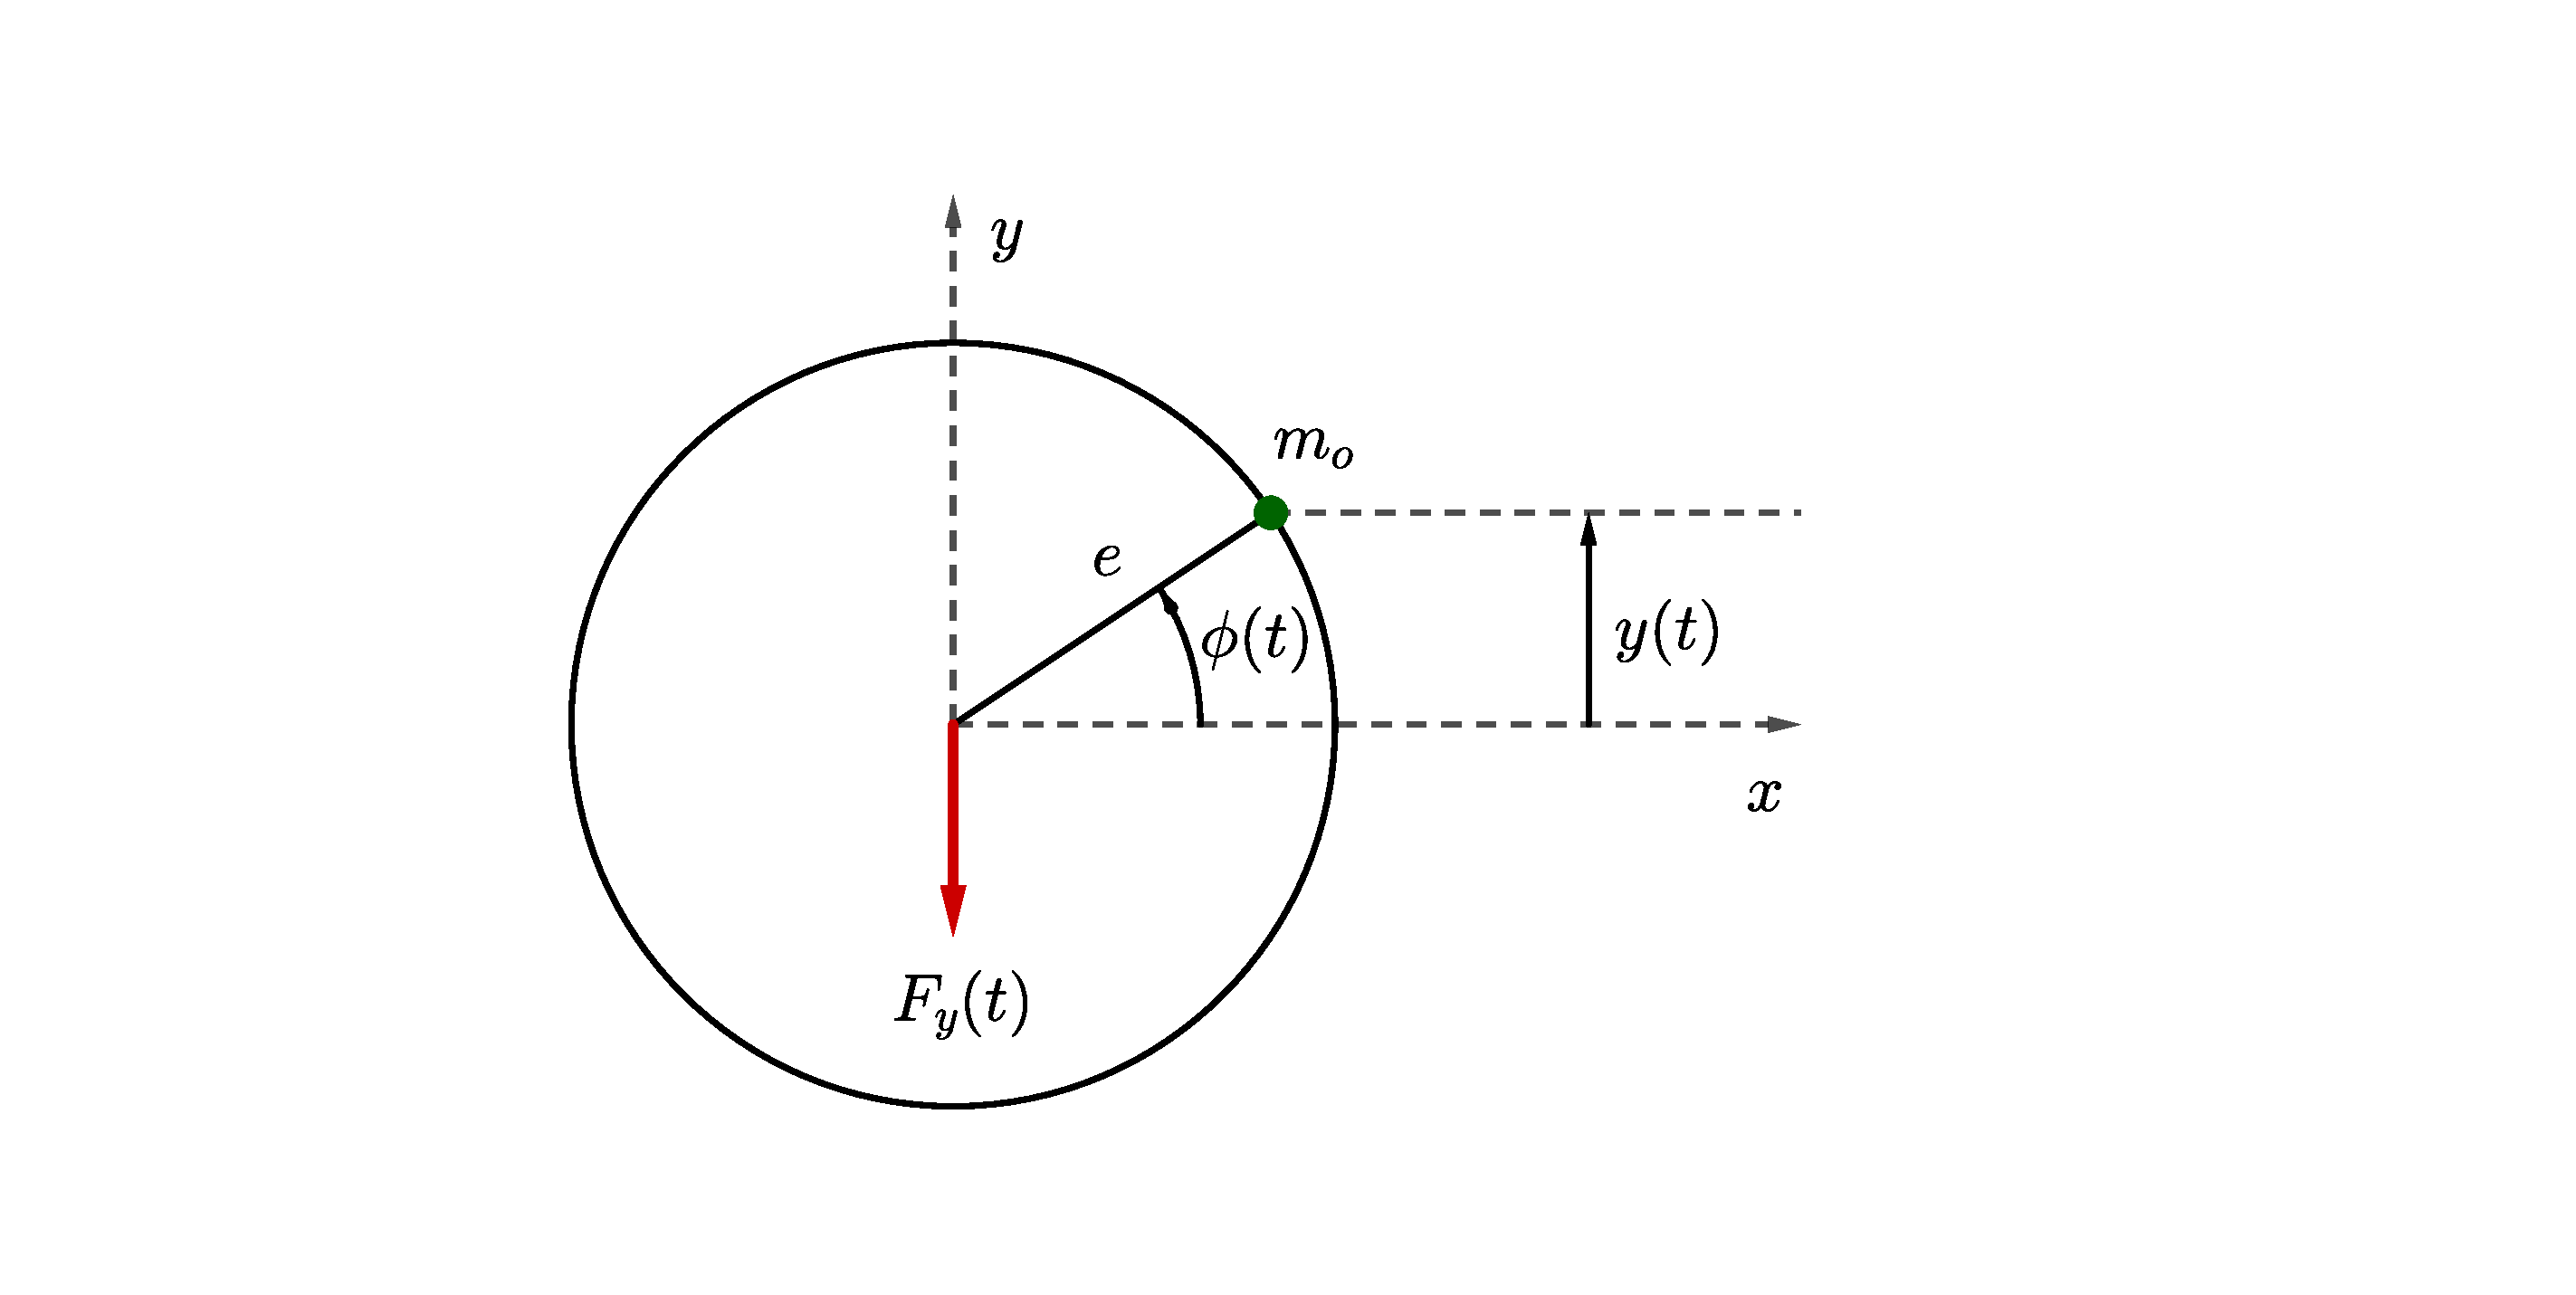
\includegraphics[width=0.7\textwidth, trim={6cm 2cm 10cm 3cm}, clip]{Imagenes/dcl_maqdes.pdf}
\caption{Diagrama de cuerpo libre de un disco desequilibrado por masa $m_0$ a una distancia $e$.}
\label{fig:dcl_maqdes}
\end{figure}

Si consideramos un desequilibrio de masa $m_0$, a una distancia $e$ del centro de rotación y rotando a una velocidad $\phi$, como se muestra en la fig. \ref{fig:dcl_maqdes}, la componente vertical de la fuerza centrífuga $F(t)$ es:
\begin{equation}
	F_y(t) = m_0\ddot{y}(t)
\end{equation}
Tomando el centro de rotación como el punto cero del sistema de coordenadas y que la aceleración angular es distinta de cero, entonces las coordenadas de posición, velocidad y aceleración quedan de la siguiente manera:
\begin{gather*}
	y(t) = e \sin \phi\\
	\dot{y}(t) = e \dot{\phi}\cos \phi\\
	\ddot{y}(t) = e(\ddot{\phi}\cos\phi - \dot{\phi}^2\sin\phi)
\end{gather*}
Por lo tanto, la ecuación \ref{eq:vib_forzadas}, muestra la fuerza centrífuga en dirección al eje $y$ cuando una masa desbalanceada $m_0$ gira a una velocidad angular $\dot{\phi}$ y su aceleración angular es $\ddot{\phi}$.
\begin{equation}\label{eq:vib_forzadas}
	F_y(t) = m_0e(\ddot{\phi}\cos\phi- \dot{\phi}^2\sin\phi)
\end{equation}

\subsection{Derivación de las ecuaciones de movimiento}
Es el proceso en el que se representan todos los detalles importantes del sistema con el objetivo de derivar las ecuaciones que  rigen el comportamiento del mismo. Para esto, los métodos existentes son la ley de movimiento de Newton, el principio de D\texttt{'}\kern-0.3em Alembert y principio de conservación de la energía. Los primeros, vistos en la sección \ref{sec:ec_mov}, se utilizan a través de un diagrama de cuerpo libre y la correcta identificación de las fuerzas y momentos que actúan sobre un cuerpo. Por otra parte, el método de conservación de la energía tiene la capacidad de derivar las ecuaciones de movimiento de un cuerpo sin la necesidad de recurrir a un diagrama de cuerpo libre, es decir, no se requiere identificar fuerzas ni momentos en el sistema. Éste método se verá en mayor profundidad en la sección \ref{sec:metodo_energia}.

Si consideramos un sistema amortiguado forzado y de un solo grado de libertad, $x(t)$ o $\theta(t)$ según sea el caso, entonces la ecuación que describe el movimiento tendrá la siguiente forma:
\begin{subequations}
\begin{align}
	m\,\ddot{x}(t) + c\,\dot{x}(t) + k\,x(t) = F(t) \label{eq:onedeglineal_damp}\\
	I\,\ddot{\theta}(t) + c\,\dot{\theta}(t) + k\,\theta(t) = M(t) \label{eq:ondegangular_damp}
\end{align}
\end{subequations}
Tanto la ecuación lineal (ec. \ref{eq:onedeglineal_damp}) y angular (ec. \ref{eq:ondegangular_damp}) son el resultado de derivarlas a través de cualquiera de los métodos expuestos anteriormente.  
 
\subsection{Sistema de múltiples grados de libertad}
El número de grados de libertad de un sistema es la cantidad de parámetros independientes necesarios para definir los movimientos que posee cada masa involucrada en el sistema. Para cada grado de libertad de una masa, corresponde una coordenada $x_i(t)$, describiendo su movimiento en esa dimensión. La fig. \ref{fig:dof} muestra las posibilidades de movimiento de un elemento de masa $m$ que no está sometido a ninguna restricción.

\begin{figure}[h]
\centering
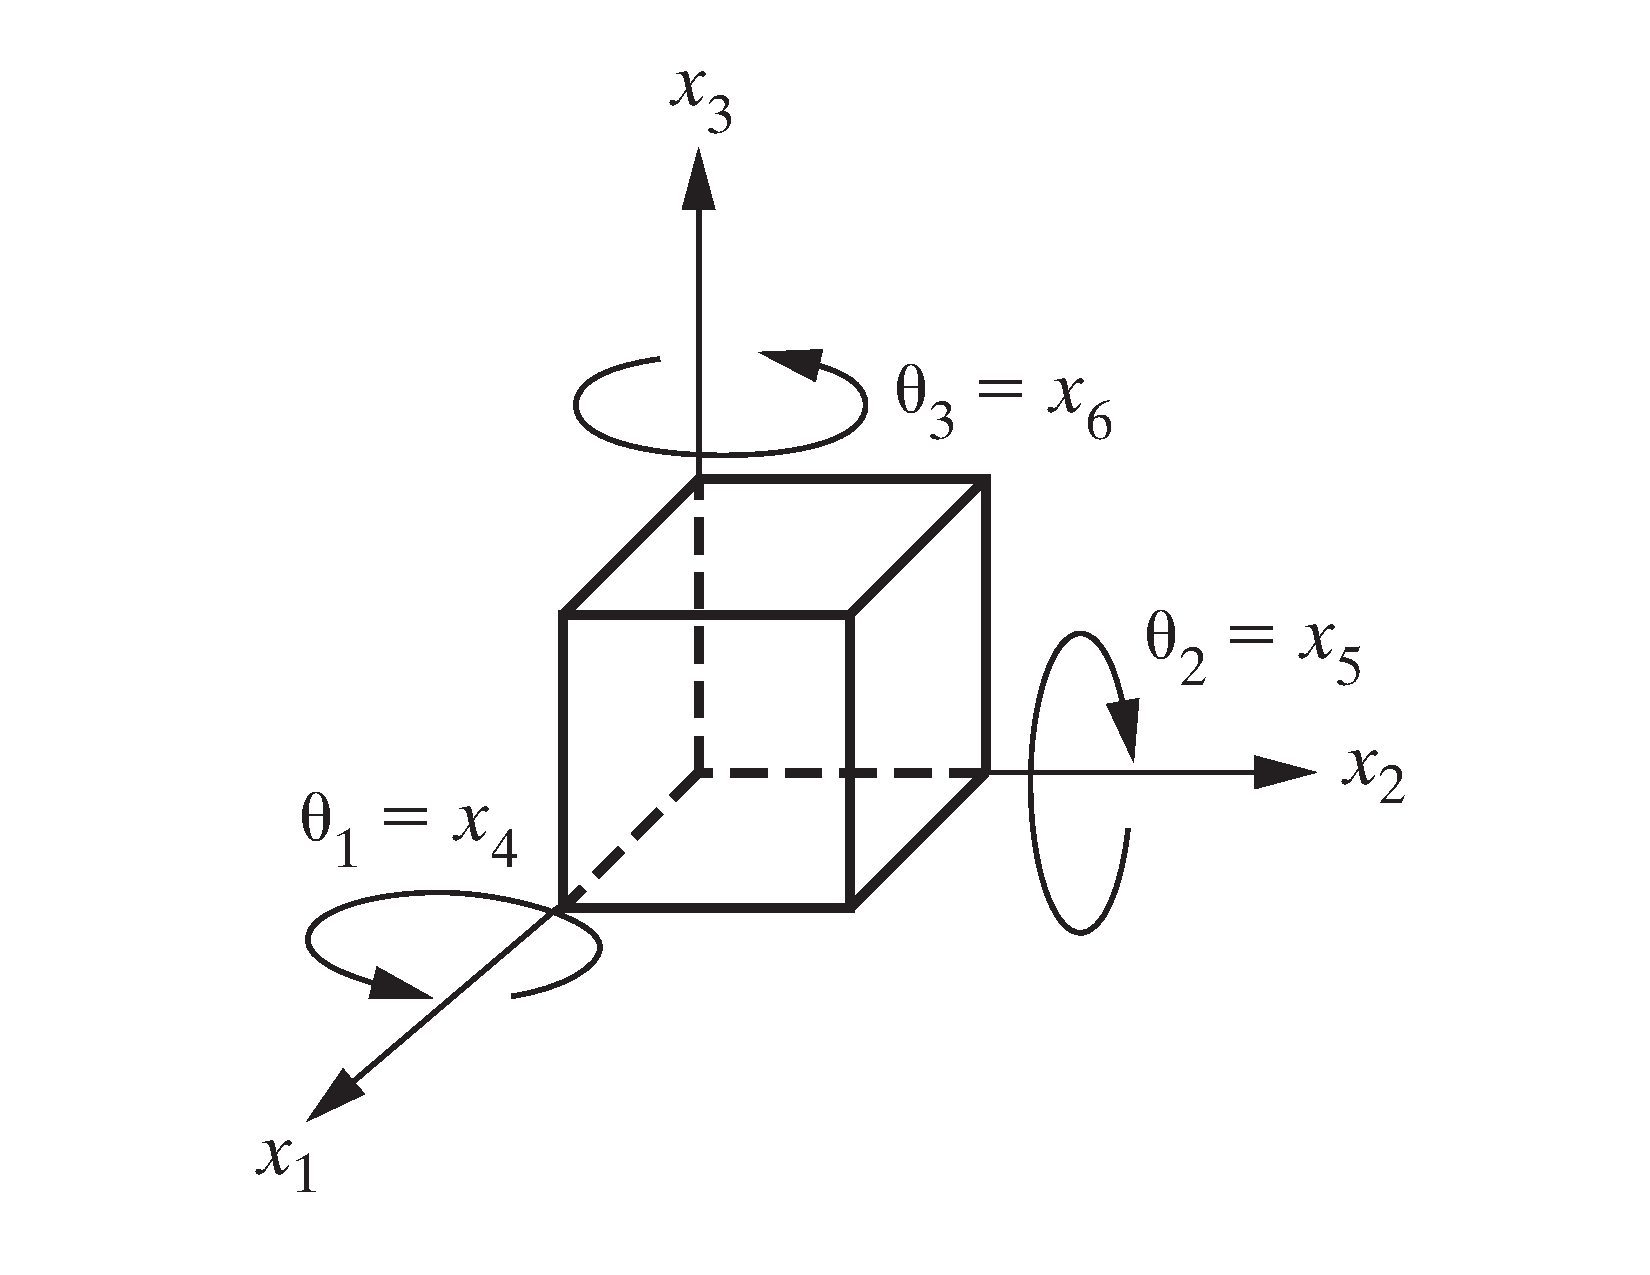
\includegraphics[width=0.5\linewidth]{Imagenes/dof.pdf}
\caption{Todos los posibles grados de libertad que puede tener una masa, los cuales se dividen en 3 grados de libertad rotacionales ($\theta_i$) y 3 lineales ($x_i$). \cite{inman2014engineering}}
\label{fig:dof}
\end{figure}

La forma de describir el movimiento de cada masa es a través del uso de matrices y vectores, de tal forma que es posible agrupar los distintos componentes que se vieron en las ecuaciones \ref{eq:onedeglineal_damp} y \ref{eq:ondegangular_damp} de un solo grado de libertad. De esta manera, las coordenadas $x_i(t)$ pueden ser escritas como un vector $\mathbf{x}(t)$ de $n \times 1$, donde $n$ es la cantidad de grados de libertad del sistema. Asimismo, se puede representar matricialmente la información de la masa del sistema y la rigidez de cada resorte, donde $\mathit{M}$ es la matriz de masas y $\mathit{K}$ es la matriz rigidez, ambas de dimensión $n \times n$. 
\begin{equation}\label{eq:multi_degree}
	\mathit{M}\mathbf{\ddot{x}}(t) + \mathit{K}\mathbf{x}(t) = 0
\end{equation}
La forma de la ec. \ref{eq:multi_degree} permite resolver un sistema de $n$ grados de libertad, por lo tanto, la forma de la matriz de masas será:
\begin{equation*}
	\mathit{M}=\text{diag}(m_1,m_2,...,m_n)
\end{equation*}
Y el vector $\mathbf{x}(t)$ es:
\begin{equation*}
	\mathbf{x}(t) = \begin{bmatrix}
	x_1(t)\\
	x_2(t)\\
	\vdots\\
	x_n(t)
	\end{bmatrix}
\end{equation*} 

\bigskip

Por otra parte, para sistemas con amortiguamiento viscoso se añade la matriz de amortiguamiento $\mathit{C}$ de dimensión $n \times n$. 
\begin{equation}\label{eq:multi_degreedamp}
	\mathit{M}\mathbf{\ddot{x}}(t) + \mathit{C}\mathbf{\dot{x}}(t) + \mathit{K}\mathbf{x}(t) = 0	
\end{equation}
Finalmente, se tendrá un sistema de $n$ ecuaciones diferenciales de segundo orden, con coeficientes constantes, cada una de las cuales requiere dos condiciones iniciales.
\begin{equation}
	\mathbf{x}(t_0) = \begin{bmatrix}
	x_{10}(t_0)\\
	x_{20}(t_0)\\
	\vdots\\
	x_{n0}(t_0)
	\end{bmatrix} \quad ; \quad \mathbf{\dot{x}}(t_0) = \begin{bmatrix}
	\dot{x}_{10}(t_0)\\
	\dot{x}_{20}(t_0)\\
	\vdots\\
	\dot{x}_{n0}(t_0)
	\end{bmatrix}
\end{equation}
Donde los valores de $\mathbf{x}(t_0)$, $\mathbf{\dot{x}}(t_0)$ y de las matrices $\mathit{M}$, $\mathit{K}$, y $\mathit{C}$ se deben conocer para poder resolver el sistema de ecuaciones. 

\subsection{Método de Lagrange}
\label{sec:metodo_energia}
El método de conservación de la energía puede ser combinado con los conceptos de trabajo virtual, lo cual lleva a que las ecuaciones de Lagrange puedan ser usadas para obtener la descripción del movimiento del sistema, incluso si son amortiguados y forzados. Sin embargo, antes de explicar su funcionamiento se debe introducir el concepto de coordenadas generalizadas.

Las ecuaciones de movimiento de un sistema vibratorio pueden estar compuestas por distintos sistemas de coordenadas, no obstante, aquellos sistemas de coordenadas independientes entre sí y de las condiciones de restricción se les llama coordenadas generalizadas, $q_j$. De igual forma, se designará como $Q_j$ a las fuerzas generalizadas que estén actuando sobre el sistema. Estas fuerzas se definen según la ec. \ref{eq:fuerza_generalizada}, donde $W_j$ es el trabajo realizado al cambiar las coordenadas generalizadas $q_j$ y $\delta q_j$ la cantidad desplazada. 
\begin{equation}\label{eq:fuerza_generalizada}
	Q_j \cdot \delta q_j = W_j
\end{equation} 

Análogo a como se ha desarrollado anteriormente, $Q_j$ puede adquirir el valor de una fuerza o momento, así como $q_j$ puede ser una coordenada de desplazamiento lineal o angular. Así mismo, $\dot{q}_j$ y $Q_j^{(n)}$ representan la velocidad generalizada y la fuerza generalizada no conservativa, respectivamente.

Con esto en consideración, el método de Lagrange define el concepto de lagrangiano $L$, como la resta entre la energía cinética $T$ y la energía potencial $U$ del sistema, ambos en términos de las coordenadas generalizadas $q_i(t)$.
\begin{equation}\label{eq:lagrangiano}
	L = T - U
\end{equation} 
Así, el método establece que para un sistema no conservativo sin amortiguamiento, la ecuación \ref{eq:der_lag} tiene la forma:
\begin{equation}\label{eq:der_lag}
	\frac{d}{dt}\left(\frac{\partial L}{\partial \dot{q}_i}\right) - \frac{\partial L}{\partial q_i} = Q_i
\end{equation}
Si se sustituye la ec. \ref{eq:lagrangiano} en \ref{eq:der_lag}, entonces se obtiene:
\begin{equation}\label{eq:der_lagconsv}
	\frac{d}{dt}\left(\frac{\partial T}{\partial \dot{q}_i}\right) - \frac{\partial T}{\partial q_i} + \frac{\partial U}{\partial q_i} = Q_i
\end{equation}
Lo que resultará en una ecuación para cada coordenada generalizada. En resumen, es importante para que el sistema esté correctamente definido la identificación de los sistemas de energía y el uso de las coordenadas generalizadas. 


\subsection{Ecuaciones de energía para un sistema con amortiguamiento y forzado}
Finalmente, es posible obtener las ecuaciones de movimiento a través del método de conservación de energía para un sistema con dos grados de libertad, forzado y con amortiguamiento viscoso. Para esto, se utilizarán los elementos mostrados anteriormente y se derivará la ecuación. Además se añadirá el efecto de la energía potencial gravitatoria, factor importante en el caso estudiado en este trabajo, donde $g$ será la gravedad. Por tanto se define según la ec. \ref{eq:e_potgrav}. 
\begin{equation}\label{eq:e_potgrav}
	U_g = mg\,q_i
\end{equation}
Por lo tanto, la energía potencial total del sistema, tendrá la siguiente forma:
\begin{equation}\label{eq:e_potencial}
	U = U_k + U_g = \frac{1}{2}k\,q_i^2 + mg\,q_i
\end{equation}

A partir de la ec. \ref{eq:der_lag}, considerando los valores de la energía cinética y potencial de las ecuaciones \ref{eq:e_cinetica} y \ref{eq:e_potencial}, es necesario añadir las fuerzas de amortiguamiento y las fuerzas externas no conservativas. La suma de estas fuerzas fue desarrollada en las secciones \ref{sec:damping} y \ref{sec:vib_forzadas}, dando como resultado las ecuaciones \ref{eq:q_ri} y \ref{eq:vib_forzadas}.
\begin{equation}\label{eq:lag_modelo}
	Q_i = F_i(t) + Q_{Ri} = F_i(t) - \frac{\partial R}{\partial \dot{q}_i} 
\end{equation}

De esta manera, una vez identificado todos los sistemas de energía y sus respectivos valores, se obtiene:
\begin{equation}
	\frac{d}{dt}\left(\frac{\partial T}{\partial \dot{q}_i}\right) - \frac{\partial T}{\partial q_i} + \frac{\partial R}{\partial \dot{q_i}} + \frac{\partial U}{\partial q_i} = F_i(t)
\end{equation}
El cual, una vez derivado y escrito de forma matricial, adquiere la siguiente forma:
\begin{equation}
	\mathit{M}\mathbf{\ddot{q}_i} + \mathit{C}\mathbf{\dot{q}_i} + \mathit{K}\mathbf{q_i} = \mathbf{F}_i
\end{equation}

\section{Plasticidad}

En el caso de metales cristalinos, la plasticidad corresponde a la deformación permanente que se produce a una escala microscópica por el movimiento de un gran número de dislocaciones producto de la aplicación de una carga sobre el material. La zona de deformación plástica es permanente, independiente del tiempo y se caracteriza por estar sobre el punto de fluencia, por lo tanto, los esfuerzos y las deformaciones dejan de ser proporcionales en la curva de esfuerzo-deformación, es decir, tienen un comportamiento no lineal . Los mecanismos que producen la deformación elástica y plástica son distintos, lo que resulta en que ambas deformaciones convivan en la deformación total, teniendo como efecto que cuando un elemento es descargado exista una recuperación de la deformación elástica. 


\subsection{Esfuerzo y deformación real}
La curva de esfuerzo-deformación ingenieril se construye a partir de dividir la carga aplicada ($P$) en la probeta por el área transversal inicial de esta, sin embargo, esto omite la deformación sufrida. Así, el esfuerzo real (\textit{true stress}, $\tilde{\sigma}$) se define como la fuerza aplicada en la probeta dividida por el área transversal en ese instante ($A$). 
\begin{equation}
	\tilde{\sigma} = \frac{P}{A}
\end{equation} 
Dada la disminución en el área $A$ el esfuerzo real crece por sobre el ingenieril y no baja al llegar al punto de esfuerzo último al considerar la estricción de la probeta. Por otro lado, la deformación real (\textit{true strain}, $\tilde{\varepsilon}$) se define como:
\begin{equation}
	\tilde{\varepsilon} = \ln\left(\frac{L}{L_i}\right)
\end{equation}
Donde $L=L_i + \Delta L$ es el largo final. Si se asume que es una deformación isocórica, es decir, no existen cambios de volumen durante la deformación plástica, entonces se tiene que $A_iL_i = AL$ y el módulo de Poisson es $\nu' = 0.5$. Al reemplazar en ambas ecuaciones, se obtiene que el esfuerzo y la deformación real es:
\begin{gather}
	\tilde{\sigma} = \sigma(1 + \varepsilon) \label{eq:true_esf}\\
	\tilde{\varepsilon} = \ln (1 + \varepsilon) \label{eq:true_strain}
\end{gather}

\subsection{Factor de corrección de Bridgman}
Cuando una probeta de acero llega al punto de estricción en un ensayo de tracción, los esfuerzos dejan de ser uniaxiales y aparecen esfuerzos en otros componentes. Esto produce que los valores de esfuerzos axiales sean mayores que los reales y deban ser corregidos. El factor que intenta corregir esta diferencia fue desarrollada por Bridgman, entregando una nueva curva de esfuerzo $\tilde{\sigma}_B$ aplicando un factor $B$ al esfuerzo real que se obtiene por la ec. \ref{eq:true_esf} \cite{dowling2013mechanical}.
\begin{equation}
	\tilde{\sigma}_B = B\tilde{\sigma}
\end{equation}
Este factor de corrección es un polinomio que se calcula a través de la deformación real que se obtiene de la ec. \ref{eq:true_strain}. Así, se define la variable $x = \log_{10} \tilde{\varepsilon}$, dando como resultado la siguiente ecuación:
\begin{equation}\label{eq:bridgman}
B = 0\text{,}0684x^3 + 0\text{,}0461x^2 - 0\text{,}205x + 0\text{,}825 
\end{equation}
La corrección se aplica en el rango $0\text{,}12 \leq \tilde{\varepsilon} \leq 3$.

\subsection{Endurecimiento isotrópico por deformación}
Se le denomina al incremento en la resistencia del material a medida que su deformación crece, luego de superar el punto de fluencia. En el caso del endurecimiento isotrópico, el esfuerzo de fluencia del material permanece centrado respecto al eje central aún cuando crezca producto de la deformación plástica, como se muestra en la fig. \ref{fig:iso_hard}.

\begin{figure}[h]
\centering
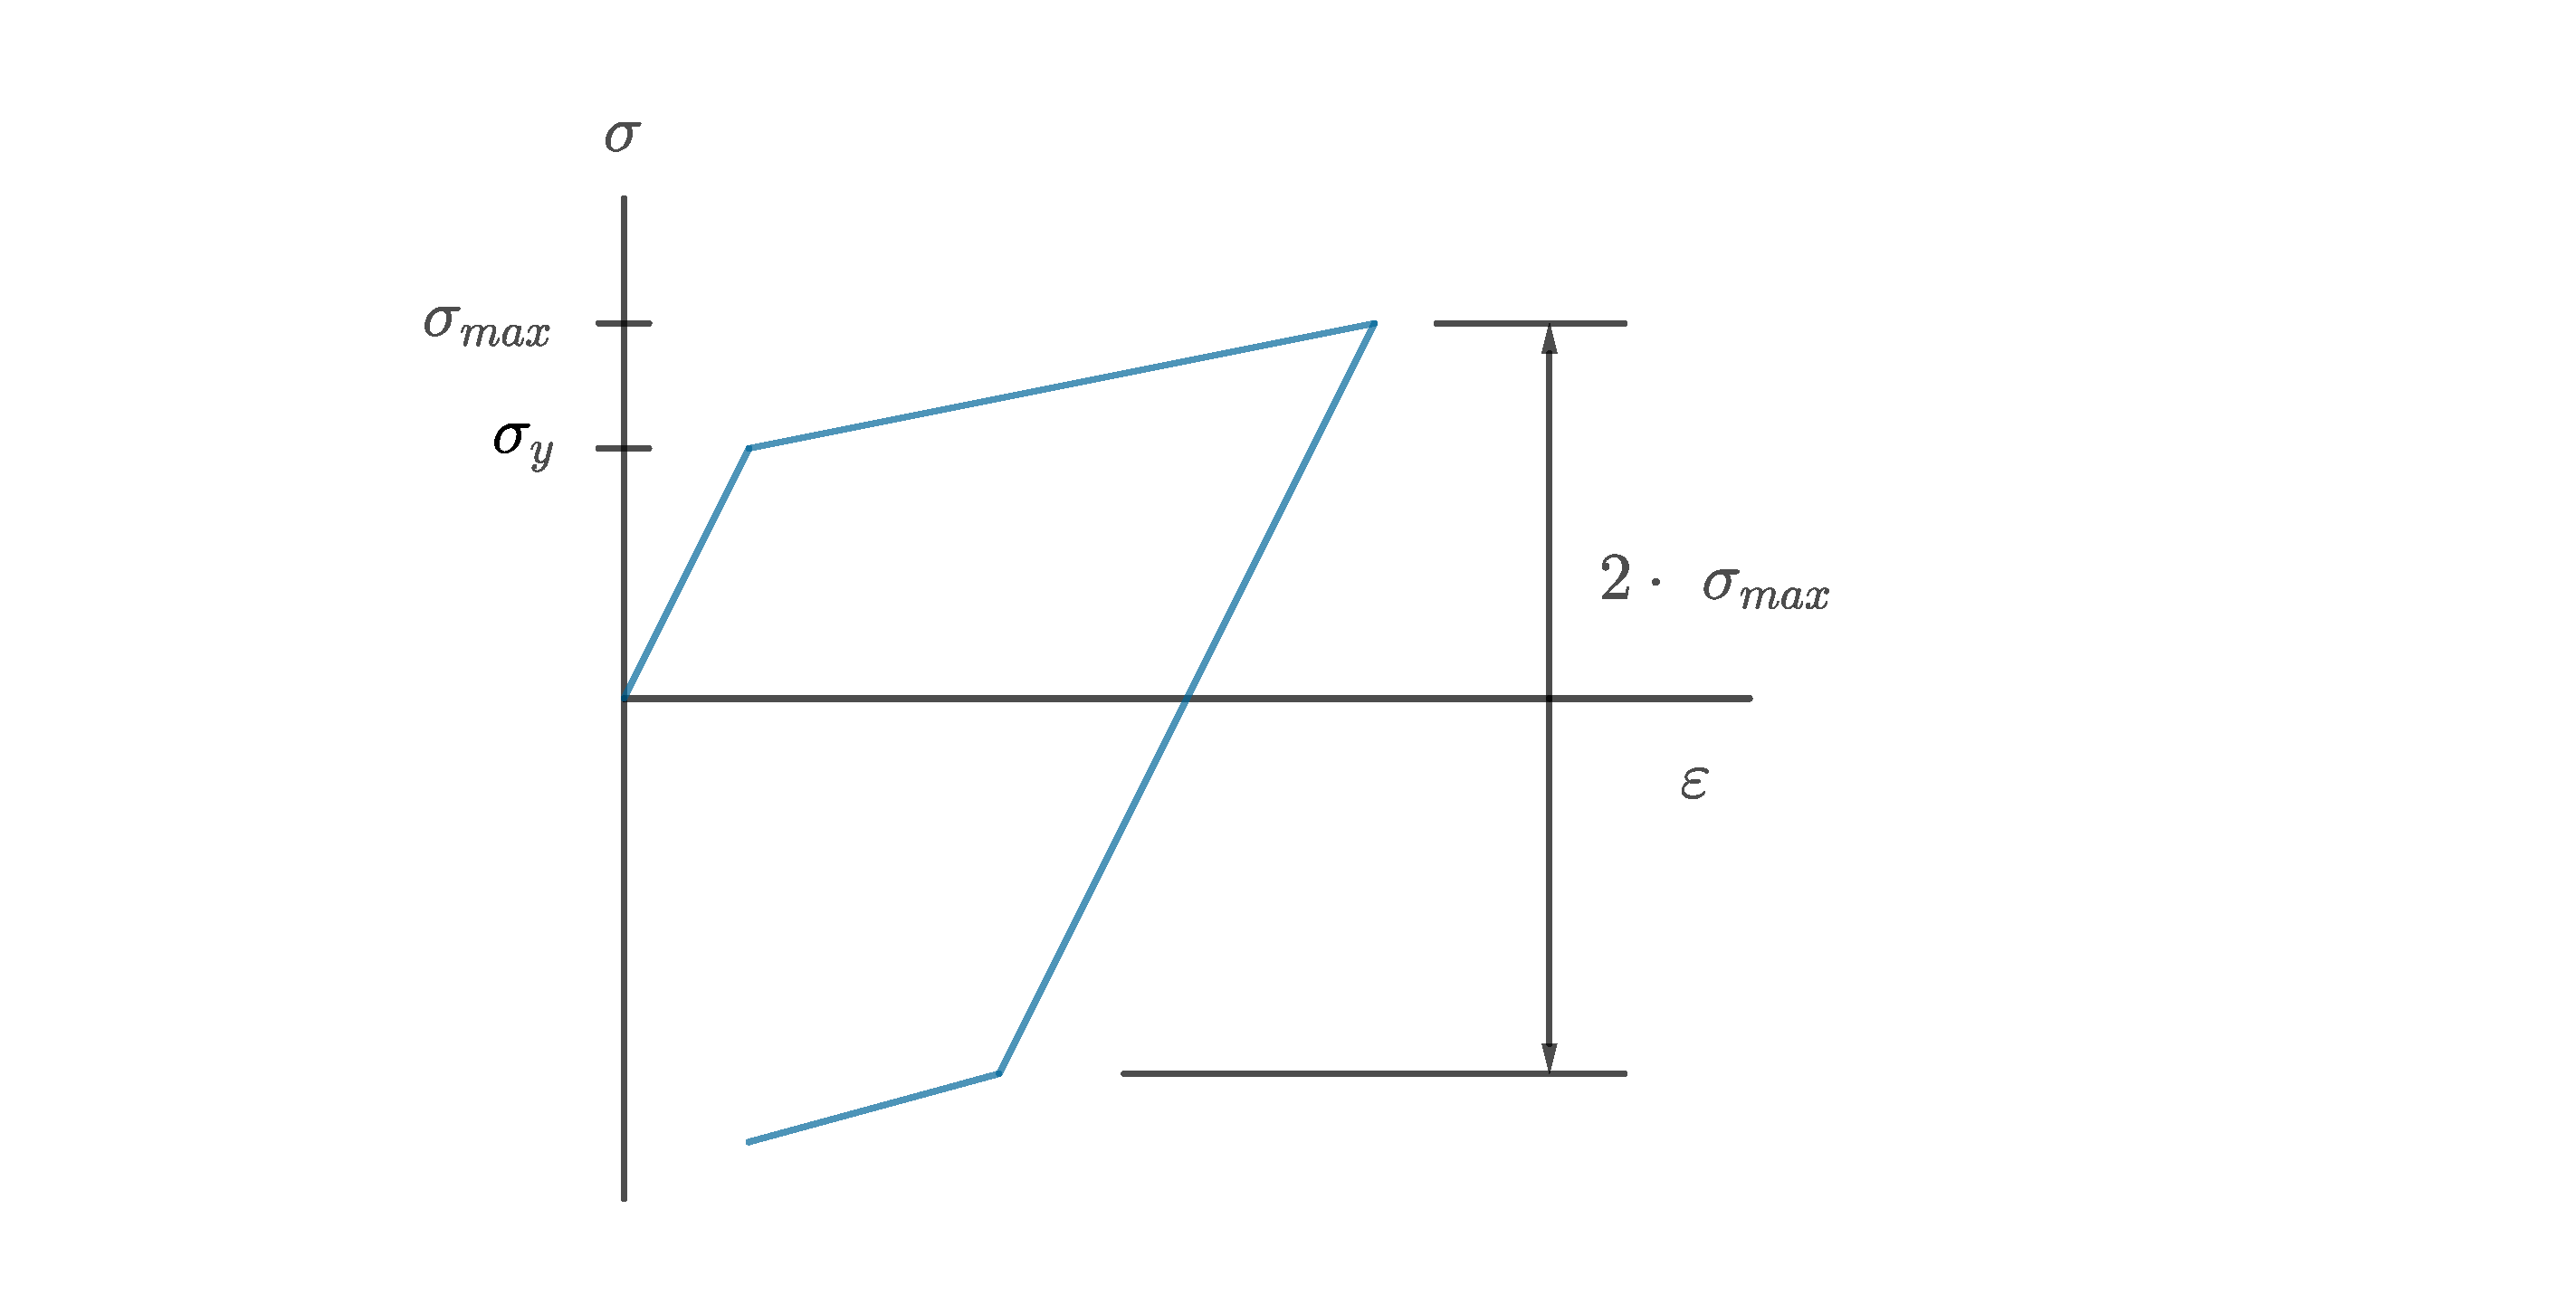
\includegraphics[width=1\linewidth]{Imagenes/iso_hard.pdf}
\caption{Endurecimiento isotrópico por deformación plástica. Se puede apreciar como se conserva la distancia del esfuerzo máximo respecto a la abscisa.}
\label{fig:iso_hard}
\end{figure}


\section{Método de elementos finitos}
El método de elementos finitos (FEM, por sus siglas en inglés) y el análisis de elementos finitos (FEA, por sus siglas en inglés) son herramientas utilizadas para proporcionar soluciones aproximadas a problemas complejos en fenómenos mecánicos. Este consiste en tomar un componente real con una estructura continua y dividirla en pequeñas subestructuras finitas de geometría mucho más simple. A este proceso se le llama  discretización, a las subestructuras elementos y a los puntos de unión nodos. 
%Las propiedades del material, las ecuaciones gobernantes y las cargas son posible aplicarlas dentro del elemento, en la cara de los mismos o incluso en los nodos. 
De esta forma, los nodos pasan a ser fundamentales al ser donde se conectan los elementos, se asignan las condiciones de frontera y se aplican las fuerza de contacto o cuerpo \cite{budynas2008shigley}. Los nodos poseen grados de libertad (DOF, por sus siglas en inglés) de la misma forma en la que se establecieron para una masa, como se puede ver en la fig. \ref{fig:dof}. Para cada nodo se escribe su correspondiente ecuación de balance y luego se puede llegar a un sistema de ecuaciones que resuelve el problema para todos los nodos simultáneamente. Las soluciones de estas ecuaciones da como resultado una aproximación del comportamiento elástico del componente a analizar. En el caso de este trabajo, este procedimiento entregará los desplazamientos de cada nodo, a partir de los cuales se pueden determinar los esfuerzos por medio de las ecuaciones constitutivas de elasticidad.

El FEA se divide en tres etapas: (a) pre-procesamiento, (b) procesamiento y (c) post-procesamiento. El primero incluye toda la preparación de los datos, la generación de la malla, la determinación del sistema coordenado, las conexiones, las condiciones de frontera, las propiedades del material y las cargas. El procesamiento en la resolución del sistema de ecuaciones y otras relaciones anexas. Para este trabajo, se deberá resolver las ecuaciones del momentum lineal para carga estática, por lo tanto. se buscarán las soluciones de la ecuación de equilibrio.  Finalmente, el post-proceso es la etapa donde se trabaja con la presentación de los resultados, es decir, los desplazamientos, la deformación y los esfuerzos requeridos son calculados durante esta etapa. 

\subsection{Mallado}
Se le llama malla a la red de elementos y nodos que discretizan un componente o una región. Para esto, los elementos pueden tener distintas formas geométricas que dependerán del tipo de problema a resolver, los grados de libertad o la capacidad computacional. La geometría dependerá de la cantidad de nodos por elementos, que para el caso de este trabajo, se utilizará el tetraedro, un elemento de 4 nodos.

Existen distintas formas de saber si la malla construida dará los resultados esperados en un tiempo óptimo. A esto se le denomina calidad de la malla, donde una mejor calidad entregará resultados más precisos en un menor tiempo. Para determinar su calidad, existen distintos parámetros que indican como está compuesta la malla generada \footnote{La definición de estos parámetros se obtuvieron de conferencias y el manual de ANSYS \cite{sharcnet_2017}\cite{ansys_2015}}.

\subsubsection{Relación de aspecto}
Es la relación entre el lado más largo y el más corto de un elemento. En este caso, un triángulo equilátero tiene un valor de 1, siendo la mejor relación posible. A medida que el triángulo se deforma, la relación entre los lados más corto y largo aumenta, como se puede ver en la fig. \ref{fig:asp_ratio}.

\begin{figure}[h]
\centering
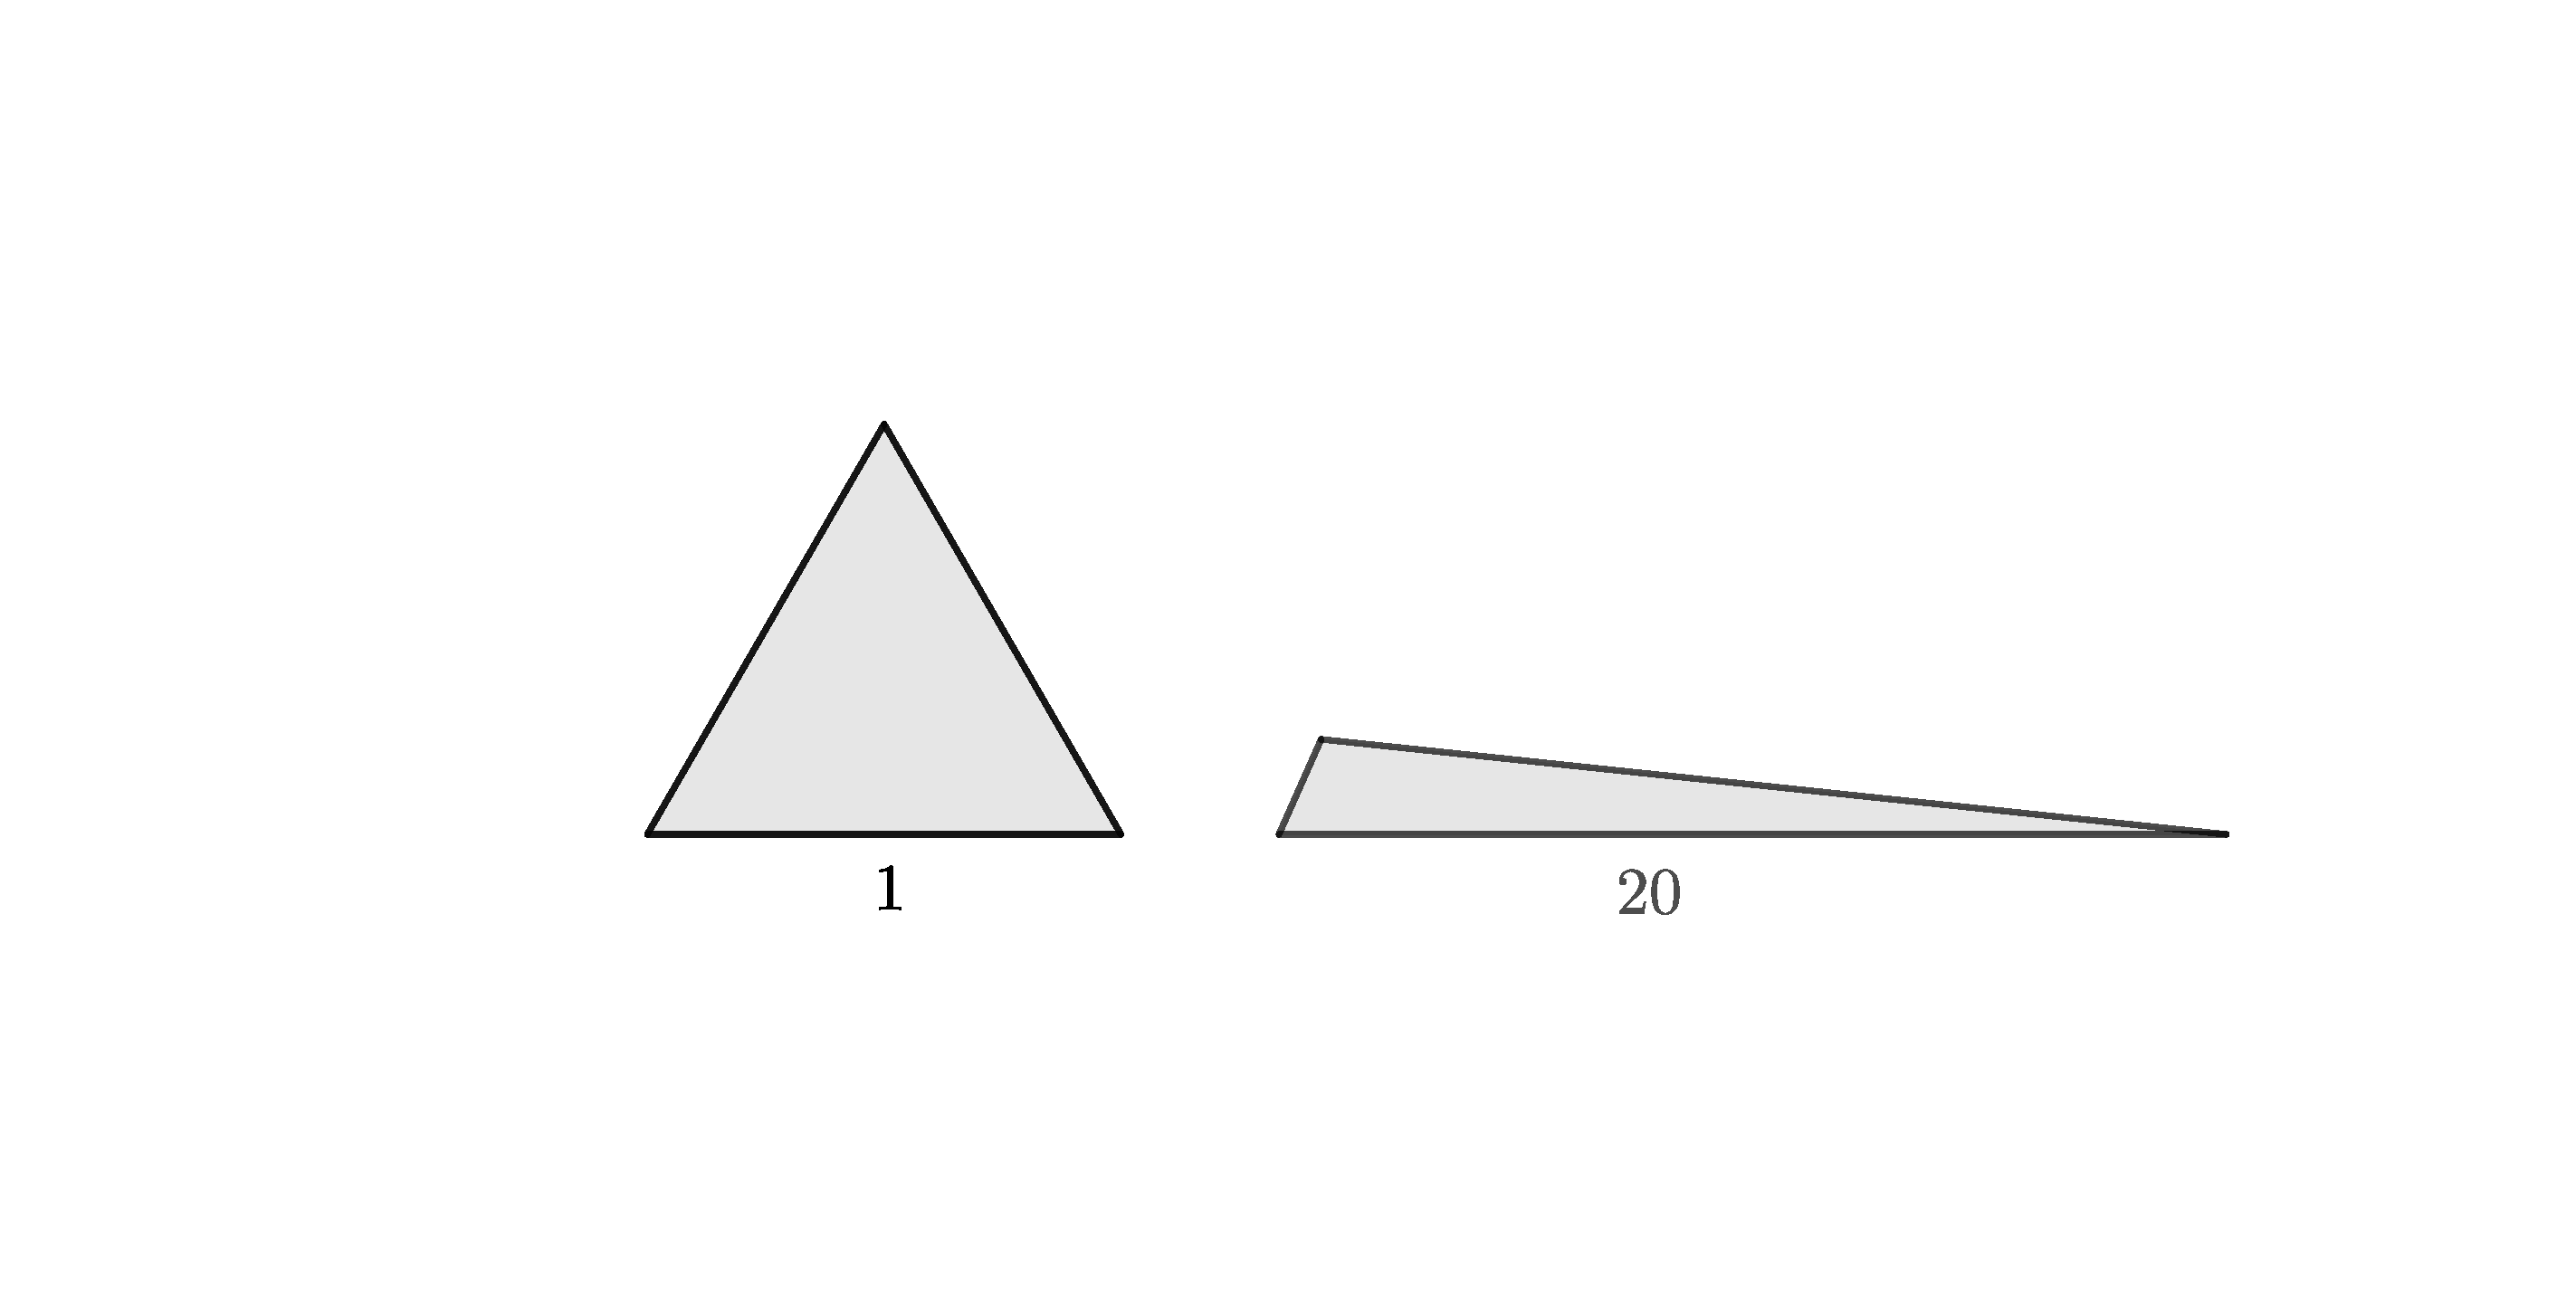
\includegraphics[width=0.5\linewidth, trim={12cm 7cm 6.5cm 7.5cm}, clip]{Imagenes/asp_ratio.pdf}
\caption{Relación de aspecto para triángulos.}
\label{fig:asp_ratio}
\end{figure}

\subsubsection{Calidad del elemento}
Se basa en la razón entre el volumen del elementos y la longitud de los bordes del elemento. Se evalúa del 1 al 0, donde 1 indica un elemento perfecto mientras que cero que el elemento no tiene volumen. Esta métrica se define como:
\begin{equation}
	\text{Calidad del elemento} = C \cdot \frac{\text{Volumen}}{\left[\sqrt{\sum \text{longitud borde}^2}\right]^3}
\end{equation}
La constante $C$ tendrá un valor definido según el tipo de elemento, para escalar su calidad de 0 a 1. Para tetraedros la constante tiene el valor de $C=124.707$, al igualar la calidad del elemento a 1 para un tetraedro regular.

\subsubsection{Calidad ortogonal}
Este parámetro se mide entre 0 y 1, donde 0 es un mal resultado y 1 el mejor. Se calcula según la ec. \ref{eq:cal_ort}, donde $\mathbf{A_i}$ es el vector normal a la cara $i$, $\mathbf{B_i}$ el vector que parte del centroide del elemento y termina en el centroide del elemento colindante a la cara $i$ y $\mathbf{C_i}$ es el vector que va desde el centroide del elemento hacia el centro de la cara $i$.

\begin{equation} \label{eq:cal_ort}
	\text{Calidad Ortogonal} = \text{MIN}\left\lbrace \frac{\mathbf{A_i}\cdot \mathbf{B_i}}{|\mathbf{A_i}||\mathbf{B_i}|} , \frac{\mathbf{A_i}\cdot \mathbf{C_i}}{|\mathbf{A_i}||\mathbf{C_i}|} \right\rbrace
\end{equation}

\subsubsection{Oblicuidad}
Es una de las medidas de calidad primarias para una malla. La oblicuidad, también llamada asimetría, determina que tan cerca está de la figura ideal está el elemento o su cara (triángulo equilátero para un tetraedro). A partir de su definición (ec. \ref{eq:skewness}), un valor 0 indica que el tamaño del elemento es igual a un triángulo equilátero y un valor de 1 indica un triángulo completamente deformado. 
\begin{equation} \label{eq:skewness}
	\text{Oblicuidad} = \frac{\text{Tamaño óptimo del elemento} - \text{Tamaño del elemento}}{\text{Tamaño óptimo del elemento}}
\end{equation}

El manual de ANSYS, entrega la tabla \ref{tab:skewness}, que sirve de guía para los valores de la oblicuidad y su respectiva calidad.

\begin{table}[]
\centering
\begin{tabular}{@{}cc@{}}
\toprule
Valor de la oblicuidad & Calidad del elemento \\ \midrule
1 & Inaceptable \\
0,9 - <1 & Muy mala \\
0,75 - 0,9 & Mala \\
0,5 - 0,75 & Buena \\
0,25 - 0,5 & Muy buena \\
>0 - 0,25 & Excelente \\
0 & Equilátero \\ \bottomrule
\end{tabular}
\caption{Lista de los rangos de los valores de la oblicuidad y la respectiva calidad del elemento. \cite{sharcnet_2017}}
\label{tab:skewness}
\end{table}

\newpage

\subsection{Ecuación del momentum lineal}

La conservación del momentum lineal es una consecuencia de la aplicación de la segunda ley de Newton. Una forma de escribir la conservación de momentum lineal es fijar un volumen de control en el espacio y considerar el flujo de momentum que entra y sale del volumen. Para esto, denominaremos \textbf{t} como la fuerza superficial por unidad de área, llamada tracción, y \textbf{b} será la fuerza del cuerpo por unidad de masa, aplicado a un volumen $v(t)$ encerrado por un área $a(t)$. Así, se obtiene:
\begin{equation}
	\int_{\text{a}(t)} \mathbf{t} \text{da} + \int_{\text{v}(t)} \rho \mathbf{b} \text{dv} = \frac{d}{dt} \int_{\text{v}(t)} \rho \mathbf{v} \text{dv}
\end{equation}
El termino \textbf{t} puede ser escrito en terminos de $\mathbf{n}\cdot \sigma$ y utilizando el teorema de la divergencia sobre la primera expresión. Luego, al hacer los arreglos necesarios y juntando terminos queda:
\begin{gather*}
	\int_{\text{v}(t)} \left\lbrace \nabla \cdot \sigma + \rho\mathbf{b} - \rho \frac{d\mathbf{v}}{dt}\right\rbrace d\text{v} = 0
\end{gather*}
De esta forma, la expresión restante escrita en forma indicial queda:
\begin{equation}
	\frac{\partial \sigma_{ij}}{\partial x_i} + \rho b_j = \rho \frac{dv_j}{dt}
\end{equation}
Obteniendose la ecuación de movimiento. Sin embargo, dado que no existen variaciones del volumen respecto al tiempo, entonces el término se desprecia y finalmente se obtiene la ecuación de equilibrio:
\begin{equation}\label{eq:mom_lin}
	\frac{\partial \sigma_{ij}}{\partial x_i} + \rho b_j = 0
\end{equation}
Expresando que la suma de las fuerzas son iguales a cero. Por lo tanto, a partir de la ec. \ref{eq:mom_lin} y las condiciones de borde de movimiento y de carga externa, es posible resolver el sistema.

\subsection{Esfuerzo y deformación}
Para esta sección, se definirá $\sigma_1$, $\sigma_2$ y $\sigma_3$ como los esfuerzos principales y $\varepsilon_1$, $\varepsilon_2$ y $\varepsilon_3$ como las deformaciones unitarias principales. 
\subsubsection{Esfuerzo y deformación unitaria de von Mises}
El esfuerzo de von Mises, llamado también equivalente, es una forma de representar un estado de esfuerzos en tres dimensiones en un valor escalar positivo. Este es calculado de la siguiente forma:
\begin{equation}
	\sigma_{vm} = \left[ \frac{(\sigma_1 - \sigma_2)^2 + (\sigma_2 - \sigma_3)^2 + (\sigma_3 - \sigma_1)^2}{2}\right]^{1/2}
\end{equation}
La deformación de von Mises total, es calculada como:
\begin{equation}
	\varepsilon_{vm,t} = \frac{1}{1+\nu'} \left[\frac{(\varepsilon_1 - \varepsilon_2)^2 + (\varepsilon_2 - \varepsilon_3)^2 + (\varepsilon_3 - \varepsilon_1)^2}{2}\right]^{1/2}
\end{equation}
Donde $\nu'$ es el coeficiente de Poisson efectivo, que se define según:
\begin{itemize*}
	\item Para la zona elástica como el coeficiente de Poisson del material $\nu$.
	\item Para la zona plástica como $\nu=0.5$
\end{itemize*}
Por lo tanto, la deformación unitaria equivalente total del material es la suma de la deformación plástica más la deformación elástica. 
\begin{equation}
	\varepsilon_{vm,t} = \varepsilon_{vm,p} + \varepsilon_{vm,e}
\end{equation}

\subsubsection{Esfuerzo máximo cortante}
El esfuerzo máximo cortante es el punto más alejado al eje de los esfuerzos normales en el círculo de Mohr, por lo tanto se define como:
\begin{equation}
	\tau_{max} = \frac{\sigma_1 - \sigma_3}{2}
\end{equation}

\subsubsection{Esfuerzo y deformación normal}
Este corresponde al esfuerzo que se produce por la carga normal a la superficie. En este caso, el esfuerzo $\sigma_{x}$ corresponde a la carga (\textit{P}) en dirección $x$ provocada sobre la superficie del plano $yz$. Por lo tanto, se define como:
\begin{equation}
	\sigma_{x} = \frac{P}{A}
\end{equation}
Así mismo, la deformación elástica en la dirección $x$ es:
\begin{equation}
	\varepsilon_{x,e} = \frac{1}{E}\left[\sigma_x - \nu (\sigma_y + \sigma_z)\right]
\end{equation}
Y la deformación plástica es:
\begin{equation}
	\varepsilon_{x,p} = \frac{1}{E_{p}} \left[ \sigma_x - 0.5(\sigma_y + \sigma_z)\right]
\end{equation}
Donde $E_{p}$ es el módulo plástico que se define como:
\begin{equation}
	E_{p} = \frac{\tilde{\sigma}}{\tilde{\varepsilon}_p}
\end{equation}
Es decir, como la pendiente provocada por una recta entre el origen y el punto de esfuerzo real y la deformación real plástica, como se ve en la fig. \ref{fig:e_p}. 
\bigskip
\begin{figure}[h]
\centering
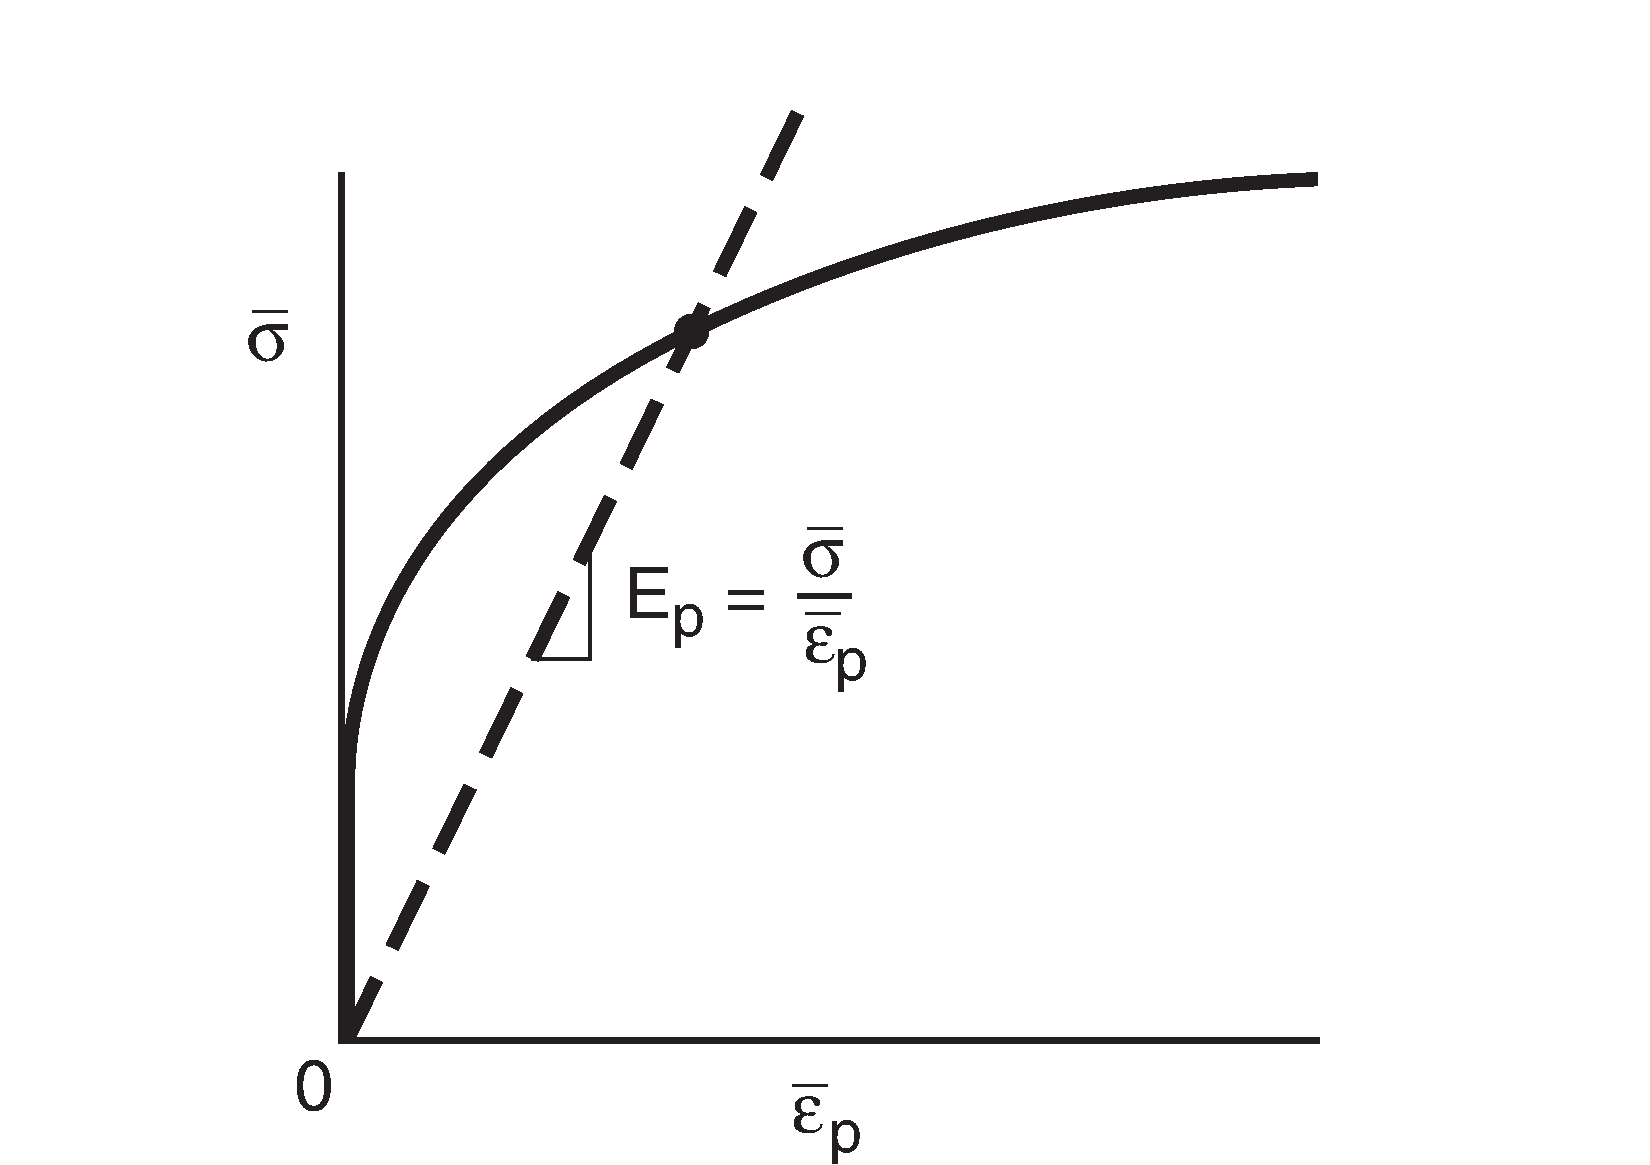
\includegraphics[width=0.6\linewidth]{Imagenes/E_p.pdf}
\caption{Definición de el módulo plástico como la pendiente entre el origen y un punto de la curva de esfuerzo yreal y deformación real plástica. \cite{dowling2013mechanical}}
\label{fig:e_p}
\end{figure}
\newpage

Sin embargo, es posible reescribir ambos módulos, $E$ y $E_{p}$, como el módulo secante $E_t$, quedando la deformación total unitaria en la dirección $x$ como:
\begin{equation}
	\varepsilon_x = \frac{1}{E_t} \left[\sigma + \tilde{\nu}(\sigma_y + \sigma_z)\right]
\end{equation}
Donde el módulo secante y coeficiente de Poisson generalizado, $\tilde{\nu}$, se definen como:
\begin{gather*}
	E_t = \frac{\tilde{\sigma}}{\tilde{\varepsilon}} \qquad ; \qquad \tilde{\nu} = \frac{\nu\sigma + 0.5E\tilde{\varepsilon}_p}{E\varepsilon}
\end{gather*}

